%%%%%%%%%%%%%%%%%%%%%%%%%%%%%%%%%%%%%%%%%%%%%%%%%%%%%%%%%%%%%%%%%%%%%%%%%%%
% Trim Size : 11in x 8.5in
% Text Area : 9.6in (include Runningheads) x 7in
% ws-ijbc.tex, 24 Jan 2010
% Tex file to use with ws-ijbc.cls written in Latex2E.
% The content, structure, format and layout of this style file is the
% property of World Scientific Publishing Co. Pte. Ltd.
%%%%%%%%%%%%%%%%%%%%%%%%%%%%%%%%%%%%%%%%%%%%%%%%%%%%%%%%%%%%%%%%%%%%%%%%%%%
%

%\documentclass[•]{•}ass[draft]{ws-ijbc}
\documentclass{ws-ijbc}
\usepackage{ws-rotating}     % used only when sideways tables/figures are used
\usepackage{epstopdf}
\usepackage{mathrsfs}
\usepackage{graphicx}
\usepackage{float}
\usepackage{bm}
\bibliographystyle{ws-ijbc}
\newcommand{\norm}[1]{\left\lVert#1\right\rVert}

\makeatletter
\newcommand*{\getlength}[1]{\strip@pt\dimexpr0.035136\dimexpr#1\relax\relax}
\newcommand{\showfont}{%
encoding: \f@encoding{},\\
family: \f@family{},\\
series: \f@series{},\\
shape: \f@shape{},\\
size: \f@size{} pt,\\
text height: \getlength{\the\textheight} cm,\\
text width:     \getlength{\the\textwidth} cm}
\makeatother


\begin{document}

\catchline{}{}{}{}{} % Publisher's Area please ignore

\markboth{Elle Musoke, Bernd Krauskopf, and Hinke M. Osinga}{A Heteroclinic Connection between Two Saddle Slow Manifolds in the Olsen Model}

\title{A Heteroclinic Connection between \\ Two Saddle Slow Manifolds in the Olsen Model}

\author{Elle Musoke, Bernd Krauskopf, and Hinke M. Osinga}


\address{Department of Mathematics, University of Auckland, Private Bag 92019\\
Auckland, 1142, New Zealand\\
elle.musoke@auckland.ac.nz}

\maketitle

\begin{history}
\received{(to be inserted by publisher)}
\end{history}

\begin{abstract}
The abstract should summarize the context, content and conclusions
of the paper. It should not contain any references or displayed
equations. Typeset the abstract in 10~pt Times Roman with
baselineskip of 12 pt, making an indentation of 1.6~cm on the left
and right margins.
\end{abstract}

\keywords{A list of 3--5 keywords are to be supplied.}
\section{Introduction}

Slow-fast dynamical systems are characterized by certain variables evolving on a fast time-scale while other variables evolve on a slower time-scale.  The separation of variables into fast and slow can be found in many systems: chemical systems, neurons, electric circuits, lasers, and predator-prey dynamics, among others, have been described by slow-fast models  \cite{BZ_reaction, Neurons, Circuits, lasers, Predator-Prey}.  This time-scale splitting arises from some vector field equations taking on much smaller values than the others in the same region of phase space.  In \cite{BZ_reaction}, oscillations in the Belousov-Zhabotinsky reaction arise as a consequence of time-scale splitting.  Slow-fast models for neurons are studied in \cite{Neurons} in which different time-scales result in neural excitability.  One of the most famous slow-fast systems is presented in \cite{Circuits} in which time-scale splitting again causes oscillations in an electronic circuit.  Lasers can also be modelled with slow-fast systems as shown in \cite{lasers} which investigated interspike interval length.  A more ecological example can be found in \cite{Predator-Prey} which uses a slow-fast model to investigate the effect of a changing predator diet on predator-prey dynamics.  Oscillatory behaviors that have the potential to be initiated by the multiple-time-scales of slow-fast systems are of significant interest by reason of their ubiquity.

Previous studies exploring the mechanisms for MMOs in slow-fast dynamical systems called upon geometric singular perturbation theory (GSPT) to investigate the role of so-called slow manifolds in the MMOs' generation and organisation \cite{Vo_paper, Vo_paper2, Emily_Harvey_paper, Martin_neuron_paper, Cris_paper}.  Slow manifolds are families of trajectories on which the flow evolves on the slow time-scale.  A slow manifold may have families of trajectories that converge toward it in forward or backward time, called the stable and unstable manifolds of the slow manifold, respectively.  Slow manifolds may have both a stable and an unstable manifold in which case we say it is a saddle slow manifold.  We give a more detailed discussion of GSPT in the next section

The mechanisms responsible for the oscillatory behaviors been studied extensively by GSPT for two- and three-dimensional systems \cite{canard_explosion, lents-rapides, enlacement,singular_hopf, folded_node,three}.  Canard explosions, small-amplitude limit cycles transitioning to larger-amplitude relaxation oscillations were studied, for example, in the two-dimensional Van der Pol oscillator and the FitzHugh--Nagumo model \cite{canard_explosion, fitz-hugh-nagumo}.  In three-dimensional systems, periodic orbits (POs) with epochs of localized small-amplitude oscillations (SAOs) and epochs of large-amplitude oscillations (LAOs) have been observed \cite{BZ}.  Only the mechanisms that cause SAOs of these appropriately named mixed-mode oscillations (MMOs) are also described in \cite{MMO} for higher-dimensional systems.  In this paper, we investigate novel phenomena that arise in four-dimensional slow-fast systems which may provide insight into undiscovered mechanisms for MMOs in higher-dimensional systems.

Very few examples exist for higher-dimensional systems.  Endocrine pituitary cells were studied with a four-dimensional slow-fast model that had a two-dimensional slow manifold in \cite{Vo_paper2}.  In \cite{Emily_Harvey_paper} a three-dimensional slow manifold was studied in a four-dimensional model for calcium oscillations inside cells. In \cite{Vo_paper} a four-dimensional model for a pituitary lactotropic cell was investigated from both a two- and three-time-scale viewpoints.  From the two-time-scale perspective, the model has a three-dimensional slow manifold.  In \cite{Martin_neuron_paper} a six-dimensional model for an excitable neuron was investigated.  The model has a two-dimensional slow manifold which plays a role in the generation of oscillations in the system.  A five-dimensional model with a one-dimensional slow manifold was also investigated.  In \cite{Saeed_Paper} techniques were developed to compute stable and unstable manifolds of one-dimensional saddle slow manifolds in three-dimensional systems. In \cite{Cris_paper}, these techniques were generalised to compute a two-dimensional saddle slow manifold and its three-dimensional stable and unstable manifolds in the four-dimensional Hodgkin--Huxley model.  To our knowledge, there is no literature on the computation of three-dimensional (un)stable manifolds of one-dimensional saddle slow manifolds at this time.

We consider a prototypical four-dimensional slow-fast dynamical system that exhibits MMOs, namely, the so-called Olsen model for peroxidase-oxidase reaction \cite{Olsen}.  There are currently many versions of the Olsen model of different dimensions.  We consider the Olsen model in the form presented in \cite{Rescaling} and earlier work \cite{Rescaling_earlier_work}.  The MMO, denoted by $\Gamma$, of the Olsen model is of particular interest because it does not seem to be generated by the mechanisms for MMOs familiar from three-dimensional systems.

The classification of variables into those that evolve on a fast time-scale and those that evolve on a slow time-scale is not straightforward for the Olsen model because the variables are not consistently slow or fast over all regions of phase space.  In fact, the Olsen model nominally has three different time-scales.  We focus specifically on a parameter regime corresponding to two different time-scales with three fast and one slow variables.  In this parameter regime there exist attracting MMOs.  It was the focus in \cite{QSSA}, which reported on mechanisms for generating MMOs after a model reduction to a three-dimensional system.  Two saddle slow manifolds were computed along with their stable and unstable manifolds.  These gave insight into the formation of the MMO, as well as the cause of its particular geometry.  However, because of the assumptions used to reduce the model to a three-dimensional system, the dimensions of the stable manifold of one slow manifold and unstable manifold of the other were reduced to two in contrast to the corresponding three-dimensional manifolds in the full system.  

Examples of computing and visualising three-dimensional manifolds are in \cite{Cris_paper, Initial_conditions_volume, Invariant_tori_again, Invariant_tori}.  None of these examples are in the context of computing (un)stable manifolds of saddle slow manifolds.  Tools to implement the computation of three-dimensional manifolds are not widely used at this time and, once computed, it is difficult to see the dynamics on the manifold in lower-dimensional projections.  Due to the nature of the current computational tools available, computing the entire three-dimensional manifold would also be computationally expensive compared to the computation of two-dimensional manifolds.

In the full system, the three-dimensional stable manifold of one slow manifold and the three-dimensional unstable manifold of the other are expected to intersect generically in a two-dimensional surface of connections between the two slow manifolds.  Such a surface does not generically exist in four-dimensional systems for slow manifolds of dimension greater than one because of the possible dimensions of their stable and unstable manifolds.  The surface of connections only exists in degenerate systems of dimension lower than four.  In these cases, the stable and unstable manifolds of the saddle slow manifolds are limited to dimensions of two or lower and therefore do not typically have robust intersections of dimension two or higher.  In this research, we generalise the techniques in \cite{Saeed_Paper, Cris_paper} with the aim of computing the three-dimensional stable and unstable manifolds of the one-dimensional saddle slow manifolds in the Olsen model.  Furthermore, we use our techniques in conjunction with Lin's method to compute the intersection of the three-dimensional stable and unstable manifolds in the full four-dimensional model.  This intersection is involved in the formation and organisation of $\Gamma$ and could lead to insights about the formation and organisation of MMOs in other higher-dimensional systems.

This paper is organized as follows.  In the next section we give the necessary background from geometric singular perturbation theory (GPST) for defining the three-dimensional manifolds which are the focus of this research.  Section 3 gives definitions of the manifolds, which are then computed.  In section 4, a computation of the intersection of the manifolds from section 3 is described for the case where the time-scale parameter is greater than zero as well as for the case when the time-scale parameter is equal to zero.  Section 5 gives an analysis of differences between the manifolds computed in section 4.  Conclusions are given in section 6.

%Background section
\section{The Olsen Model}

We consider the scaled system from \cite{Rescaling}, given as the following system of ordinary differential equations
    
\begin{equation}
\begin{aligned}
\begin{cases}
\frac{dA}{dt} &= \mu - \alpha A - ABY, \\ \\
\frac{dB}{dt} &= \varepsilon(1-BX - ABY), \\ \\
\frac{dX}{dt} &= \lambda(BX - X^2 +3ABY - \zeta X + \delta), \\ \\
\frac{dY}{dt} &= \kappa\lambda(X^2 - Y - ABY),
\end{cases}
\end{aligned}
\label{equation_1}
\end{equation}
    
\noindent
where $(A, B, X, Y)\in\mathbb{R}^{4}$ are positive concentrations of chemicals.  The system parameters are represented by Greek letters that have the values given in Table 1.  These are the same values as in \cite{Rescaling}.  With the minor modification of using $\varepsilon$ for $\varepsilon_{b}$ and $\frac{1}{\lambda}$ for $\varepsilon^{2}$ for notational convenience.  The time-scaling parameters $\varepsilon$ and $\lambda$ are chosen so that we may consider $A$, $X$, and $Y$ as fast variables, and $B$ as a slow variable; see \cite{Rescaling}.

\begin{table}[t!]
\tbl{Parameters of system (\ref{equation_1}) as in \cite{Rescaling} so that $A$, $X$, and $Y$ are fast and $B$ is slow.}
{\begin{tabular}{c  c  c  c  c  c  c  c  c} \\[-2pt]
\toprule
$\alpha$ & $\delta$ & $\varepsilon$ & $\lambda$ & $\kappa$ & $\mu$ & $\zeta$ \\[6pt]
\hline\\[-6pt]
0.0912 & $1.2121 \times 10^{-5}$ & 0.0037 & 18.5281 & 3.7963 & 0.9697 & 0.9847\\[1pt]
\botrule
\end{tabular}}
\end{table}
    
The classical analysis of slow-fast systems considers two singular limits for systems with two time-scales; for example, see \cite{MMO}.  In the limit of $\varepsilon = 0$, system (\ref{equation_1}) reduces to
    
\begin{equation}
\begin{aligned}
\begin{cases}
\frac{dA}{dt} &= \mu - \alpha A - ABY, \\ \\
\frac{dX}{dt} &= \lambda(BX - X^2 +3ABY - \zeta X + \delta), \\ \\
\frac{dY}{dt} &= \kappa \lambda(X^2 - Y - ABY),
\end{cases}
\end{aligned}
\label{equation_2}
\end{equation}
    
\noindent
with $\frac{dB}{dt}=0$, meaning that $B$ is a parameter of (\ref{equation_2}).  We refer to the three-dimensional system (\ref{equation_2}) as the fast subsystem.  Performing the time rescaling $\tau = \varepsilon t$ and then considering the limit of $\varepsilon = 0$, system (\ref{equation_1}) reduces to the differential algebraic system
    
 \begin{equation}
\begin{aligned}
\begin{cases}
0 &= \mu - \alpha A - ABY, \\ \\
\frac{dB}{d\tau} &= (1-BX - ABY), \\ \\
0 &= \lambda (BX - X^2 +3ABY - \zeta X + \delta), \\ \\
0 &= \kappa \lambda(X^2 - Y - ABY).
\end{cases}
\end{aligned}
\label{equation_3}
\end{equation}
    
\noindent
The three algebraic equations in system (\ref{equation_3}) define a one-dimensional manifold, called the critical manifold, denoted $C$.

The critical manifold $C$ consists of equilibria of the fast subsystem (\ref{equation_2}), which exist in ($A$,$B$,$X$,$Y$)-space.  Their stability can be determined from the eigenvalues of the $3\times3$ Jacobian matrix of (\ref{equation_2}) evaluated at each point on the critical manifold for the appropriate value of $B$.  Points $p \in C$ at which the Jacobian of (\ref{equation_2}) has eigenvalues with non-zero real parts are called hyperbolic.  The eigenvectors associated with the eigenvalues are categorized based on the sign of the real part of the associated eigenvalue.  Eigenvectors whose associated eigenvalues have negative real parts are called stable directions of $p$ and these span the stable eigenspace $E^{s}(p)$ of $p$.  The unstable directions and the unstable eigenspace $E^{u}(p)$, can be defined similarly by the eigenvectors associated with eigenvalues having positive real part.  Note that the dimensions of the stable and unstable eigenspaces are equal to the number of eigenvalues with negative and positive real parts, respectively.  Equilibria at which the Jacobian has eigenvalues with zero real part are called non-hyperbolic and these correspond to bifurcations of system (\ref{equation_2}) \cite{The_Kuz} .

\begin{figure}[!t]
\centering
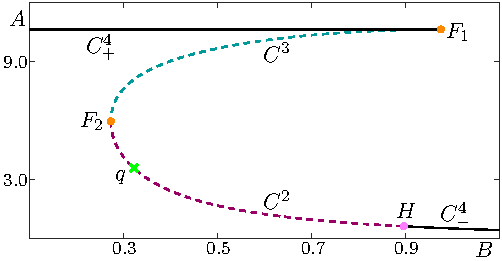
\includegraphics[]{./figures/MKMO_1.pdf}
\caption{Physically relevant branches $C^2$, $C^3$, $C^4_\pm$ of the critical manifold of (\ref{equation_1}) shown in projection onto the ($B$,$A$)-plane.  Branches $C^2$ (dashed, raspberry curve) and $C^3$ (dashed, teal curve) consist of saddles of (\ref{equation_2}) and $C^4_\pm$ (solid, black curve) consist of attractors of (\ref{equation_2}).  Superscripts indicate the dimension of the stable eigenspace of the branch and subscripts are used to distinguish between the two branches of attractors.  Branches are divided by saddle-node bifurcation points $F_1$ and $F_2$ (orange dots) and a Hopf point $H$ (pink dot).  Also shown is the saddle equilibrium $q$ (green cross) of (\ref{equation_1}) on $C^2$.}
\label{figure_1}
\end{figure}

The critical manifold $C$ in ($A$,$B$,$X$,$Y$)-space is divided into branches by bifurcation points of the fast subsystem (\ref{equation_2}), so that points on each branch have the same dimensions of stable and unstable eigenspaces.  In other words, the branches of $C$ are one-parameter families in $B$ of hyperbolic equilibria of system (\ref{equation_2}).  We define the stable eigenspace $E^s(C^i)$ of a branch $C^i$ as the collection of stable eigenspaces of all the points on the branch.  Hence, the dimension of $E^s(C^i)$ is one higher than the dimension of the stable eigenspace of each point on the branch. 

Four branches of $C$ lie in the physically relevant region where all phase-space variables are positive, and two of these are attracting.  The four branches are shown in Figure \ref{figure_1} in projection onto the ($B$,$A$)-plane.  In our notation for branches, superscripts indicate the dimension in ($A$,$B$,$X$,$Y$)-space of the stable eigenspace of the branch.  Further, we use subscripts to distinguish the two branches on which equilibria have three-dimensional stable eigenspaces, that is, are attracting.   The uppermost branch, denoted $C^4_+$ (solid, black curve), consists of stable equilibria of (\ref{equation_2}).  It is separated from the branch of saddle equilibria, denoted $C^3$ (dashed, teal curve), by a very sharp fold at the point $F_1$ (orange dot) at $B \approx 0.956$.  Folds of the critical manifold correspond to saddle-node bifurcations of system (\ref{equation_2}) with respect to the parameter $B$, these are points at which one of the real eigenvalues of the Jacobian changes sign.  Another fold at $B \approx 0.273$, denoted $F_2$ (orange dot), separates $C^3$ from a lower branch of saddle equilibria, denoted $C^2$ (dashed, raspberry curve).   The branch $C^2$ ends at a Hopf bifurcation $H$ (pink dot) at $B \approx 0.897$, where two complex-conjugate eigenvalues of the Jacobian pass through the imaginary axis of the complex plane.  To the right of $H$, there is again a stable branch of equilibria denoted $C^4_-$ (solid, black curve).

The point $q$ (green cross) on $C^2$ in Figure \ref{figure_1} is an equilibrium of system (\ref{equation_3}) and is, hence, an equilibrium for the full system (\ref{equation_1}).  The equilibrium $q$ has a two-dimensional stable and two-dimensional unstable manifold, denoted $W^s(q)$ and $W^u(q)$, respectively.  The manifolds $W^{s}(q)$ and $W^{u}(q)$ consist of trajectories in ($A$, $B$, $X$, $Y$)-space that converge to $q$ in forward and backward time respectively.  To the right of $W^u(q)$, in the ($B$, $A$)-projection, the flow is from right to left near $C^2$.  To the left of $W^u(q)$, in the ($B$, $A$)-projection, the flow is from left to right near $C^2$.  The manifolds $W^{s}(q)$ and $W^{u}(q)$ can be computed with the methods in \cite{Red_book}; They are not depicted in Figure \ref{figure_1}, but are shown in Figure \ref{figure_10}.

Our interest is in the branches $C^3$ and $C^2$ because they are saddle objects of different types and are crucial for organising the phase space.  These branches of the critical manifold are invariant for $\varepsilon = 0$, but not for $\varepsilon > 0$.  However, they do persist as locally invariant manifolds, called slow manifolds \cite{Fenichel}.  The associated slow manifolds are traditionally denoted $S^3_\varepsilon$ and $S^2_\varepsilon$ but, for notational convenience, we drop the subscript indicating dependence on $\varepsilon$ and refer to these slow manifolds for $\varepsilon > 0$ simply as $S^3$ and $S^2$.  The slow manifolds $S^3$ and $S^2$ have the same dimension and stability as $C^3$ and $C^2$ and lie at an $O(\varepsilon)$ Hausdorff distance from $C^3$ and $C^2$, respectively.  (For a definition of Hausdorff distance see, e.g., \cite{Hausdorff_Distance}.)  In particular, $S^3$ converges to $C^3$ as $\varepsilon \rightarrow 0$.  similarly, $S^2$ converges to $S^3$ as $\varepsilon \rightarrow 0$  Orbit segments that lie on a slow manifold remain slow for $O(1)$ time with respect to the slow time-scale.  It follows that any trajectory that remains slow for an $O(1)$ amount of slow time can be considered (to be on) a slow manifold.  However, trajectories on a slow manifold may eventually become fast. Due to their finite-time nature, slow manifolds are not unique; however, any two slow manifolds lie exponentially close to each other in a suitable $O(\varepsilon)$ neighbourhood of the associated branch on the critical manifold \cite{Fenichel}.  We select representatives $S^3$ and $S^2$ as the slow manifolds that remains slow for the longest amount of time; see the numerical set-up in section 3.

The Stable Manifold Theorem tells us that each $p \in C^3$ has a stable and an unstable manifold that are tangent to and have the same dimensions as $E^{s}(p)$ and $E^{u}(p)$, respectively \cite{Perko_book}.  We denote the stable manifold of a point $p \in C^3$ by $W^{s}(p)$ and its unstable manifold by $W^{u}(p)$.  We can then define the collection of stable manifolds for $p \in C^3$ as $W^{s}(C^3) = \bigcup_{p \in C^3} W^{s}(p)$, which is a three-dimensional manifold tangent to $E^s(C^3)$.  We can similarly define the three-dimensional unstable manifold $W^{u}(C^2)$ of $C^2$ which is tangent to $E^u(C^2)$.

According to Fenichel Theory, for $\varepsilon > 0$, the manifold $W^{s}(C^3)$ also persists in an $O(\varepsilon)$ neighbourhood as a three-dimensional local stable manifold $W^{s}_{loc}(S^3)$ of $S^3$.  The local stable manifold $W^{s}_{loc}(S^3)$ consists of families of trajectories that have a fast approach to $S^3$ then remain close to $S^3$ for $O(1)$ slow time.  The global stable manifold $W^{s}(S^3)$ can be obtained by extending $W^{s}_{loc}(S^3)$ backward in time.  The three-dimensional unstable manifold $W^{u}(S^2)$ associated with $S^2$ is similarly defined for backward time.  Again, due to the finite-time nature of the definitions for the three-dimensional manifolds $W^{s}(S^3)$ and $W^{u}(S^2)$, they are not unique.  To select unique representatives, we consider two-parameter families of orbit segments that remain slow for the longest amount of time, subject to boundary conditions.  In the next section, we describe our computational set-up in detail.  
 
 %Saddle slow manifold section   
 \section{Computation of saddle slow manifolds and their (un)stable manifolds}

In \cite{Saeed_Paper} algorithms are presented for the computation of a one-dimensional saddle slow manifold and its (un)stable manifolds in a three-dimensional system.  We build on this work to define and compute unique representatives $S^3$ and $S^2$ as well as their stable and unstable manifolds, respectively.

\subsection{Definition of $S^3$}    
We define the slow manifold $S^3$ with respect to a closed interval $[B_{\mathrm{in}},B_{\mathrm{out}}]$ for the slow variable $B$.  The values for $B_{\mathrm{in}}$ and $B_{\mathrm{out}}$ are chosen such that $[B_{\mathrm{in}},B_{\mathrm{out}}] \subset (B_{F_1}, B_{F_2})$, where $B_{F_1}$ and $B_{F_2}$ are the $B$-values of the fold points $F_1$ and $F_2$, respectively.  Hence, for each $B_p \in [B_{\mathrm{in}},B_{\mathrm{out}}]$ there is a unique point $p=(p_A,p_B,p_X,p_Y) \in C^3$ such that $p_B = B_p$.  In the three-dimensional subsection $\{ \omega \in \mathbb{R}^4 \; | \; \omega_B=B_p\}$ we define a solid three-sphere $D^s_\delta(B_p)$ with radius $\delta$ and centre $p$ , given formally by

\begin{equation*}
D^s_\delta(B_p)=\{w \in \mathbb{R}^4 \; | \; w_B = B_p, \left\lVert w-p \right\rVert \leq \delta\}.
\end{equation*}    
\noindent
The union 
\begin{equation*}
\mathscr{D}^s = \bigcup\limits_{B_p \in [B_{\mathrm{in}}, B_{\mathrm{out}}]}^{} D^s_\delta(B_p)
\end{equation*}


\noindent
forms a four-dimensional compact cylinder.  The superscript $s$ indicates that the radius $\delta$ is small, but it needs to be of $O(\varepsilon)$ to ensure that $S^3$ lies in $\mathscr{D}^s$.  The one-parameter family of orbit segments that enter $\mathscr{D}^s$ via $D_\delta(B_{\mathrm{in}})$ are candidates for $S^3$.   To select a representative $S^3$ we require that the orbit segment representing $S^3$ has maximal integration time in $\mathscr{D}^s$ while satisfying appropriate boundary conditions.  Our choice of boundary conditions is explained in section 3.2.
    
Figure \ref{figure_2} illustrates this definition with an enlargement of Figure \ref{figure_1} near the branch $C^3$, where we now sketch the relevant elements of this definition in projection onto the $(B,A)$-plane. The selected slow manifold $S^3$, enters $\mathscr{D}^s$ at $D^s_\delta(B_{\mathrm{in}})$ and exits at $D^s_\delta(B_{\mathrm{out}})$ (purple disks).

\begin{figure}[!t]
\begin{center}
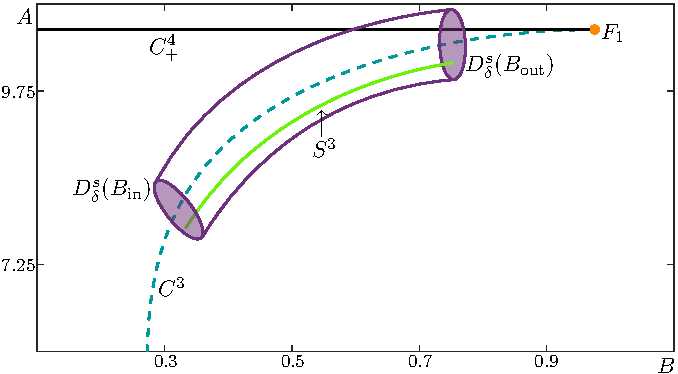
\includegraphics{./figures/MKMO_2.pdf}
\end{center}
\caption{A sketch of the selected slow manifold $S^3$ (green curve) projected onto the ($B$,$A$)-plane.  The slow manifold $S^3$ is defined by having the longest integration time while entering and exiting  $D^s_\delta(B_{\mathrm{in}})$ and $D^s_\delta(B_{\mathrm{out}})$ (purple disks) at either end of a four-dimensional cylinder.  Also shown are $C^3$, $C^4_+$, and $F_1$.}
\label{figure_2}
\end{figure}

\subsection{Computation of $W^{s}(S^3)$ and  $S^3$}

Since $W^{s}(S^3)$ is three dimensional it is challenging to compute and difficult to visualise.  In fact, $W^{s}(S^3)$ can be represented as a two-parameter family of orbit segments that enter $\mathscr{D}^s$ at $D^s_{\delta}(B_p)$ for some $B_p \in [B_{\text{in}}, B_{\text{out}}]$, and remain inside $\mathscr{D}^s$ for $O(1)$ slow time.  A natural way forward is to consider $W^{s}(S^3)$ as a one-parameter family of two-dimensional submanifolds.  These submanifolds can be computed by generalizing the approach in \cite{Saeed_Paper} based on a two-point boundary value problem (2PBVP) set-up and continuation, which can then be implemented in the continuation package \textsc{Auto} \cite{AUTO}.  

Similarly to $S^3$, we select and approximate a specific candidate for $W^{s}(S^3)$ by requiring that each orbit segment approaching $S^3$ has maximal integration time inside $\mathscr{D}^s$ and satisfies appropriate boundary conditions.  We now turn to the computation of the three-dimensional manifold $W^{s}(S^3)$ in the region where a corresponding two-dimensional stable manifold was investigated in the reduced model of \cite{QSSA}.

To select a submanifold we first define a two-dimensional plane $\Sigma$ that is transverse to the flow and to $E^u(C^3)$.  We can define $\Sigma$ by fixing $A$ and either $X$ or $Y$.  A smooth, one-parameter family of orbit segments of (\ref{equation_1}) is then given by the property that they begin in $\Sigma$, enter $\mathscr{D}^s$ at $D^s_{\delta}(B_p)$ for some $B_p \in [B_{\text{in}}, B_{\text{out}}]$, and remain inside $\mathscr{D}^s$ for $O(1)$ slow time.  We denote by $W^{s}_{\Sigma}$ the collection of the parts of these orbit segments that enter $\mathscr{D}^s$ in the fast direction.  The later parts that evolve mostly in the $B$-direction inside $\mathscr{D}^s$ for $O(1)$ slow time are approximate segments of $S^3$.  If such a later part of the orbit segment includes a fast exit from $\mathscr{D}^s$, the fast part lies on the unstable manifold $W^{u}(S^3)$ of $S^3$ in good approximation.

\begin{figure}[t!]
\centering
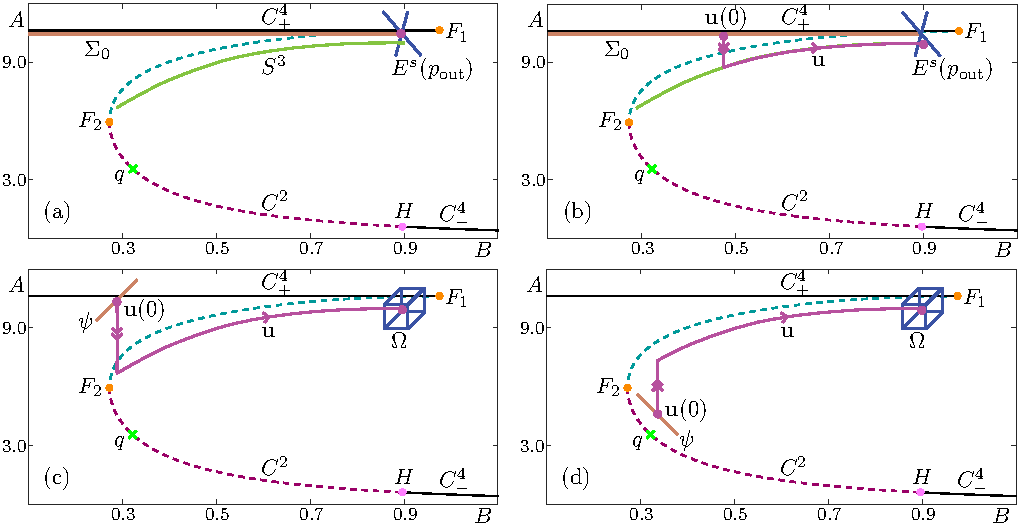
\includegraphics[]{./figures/MKMO_3.pdf}
\caption{A sketch in projection onto the ($B$,$A$)-plane of the numerical set-up for the computation of submanifolds of $W^s(S^3)$.  Also shown are $C^2$, $C^3$, $C^4_\pm$, $F_1$, $F_2$, $H$ and $q$.  Panel (a) shows a sketch at the start of the first homotopy step for computing $W^{s}_{\Sigma_0}$ with $S^3$ (green curve), $E^s(p_{\text{out}})$ (blue cross), and the plane $\Sigma_0$ (mocha line) defined by the $A$- and $Y$-coordinates of the point $p_{\text{out}}$.  Panel (b) shows a representative orbit segment $\mathbf{u}$ (magenta curve) of the first homotopy step.  Panel (c) shows an illustration of the selection of $\mathbf{u}$ with maximal integration time that starts at $\psi$ (mocha line) and ends on $\Omega$ (blue cube); here the one-dimensional subset $\psi \subset \Sigma_0$ is defined by fixing $B = B_{\text{in}}$ and $\Omega$ is spanned by $E^s(p_{\text{out}})$ and a vector in the $B$-direction. Panel (d) is a sketch of the selection of a different submanifold $W^{s}_{\Sigma}$ for $\Sigma$ on the other side of the critical manifold.}
\label{figure_3}
\end{figure}


We compute the submanifold $W^s_{\Sigma}$ as a one-parameter family of orbit segments $\mathbf{u} = \{\mathbf{u}(s) \;|\; 0 \leq s \leq 1 \}$ of the rescaled system

\begin{equation}
\frac{d\mathbf{u}}{ds} = TF(\mathbf{u}),
\label{equation_4}
\end{equation}
    
\noindent
where $\mathbf{u}(s) = (A(s), B(s), X(s), Y(s)) \in \mathbb{R}^4$ is the vector of chemical concentrations, $F$ is the right-hand side of (\ref{equation_1}) and $T$ is the total integration time on the fast time-scale.  Orbit segments $\mathbf{u} \in W^s_{\Sigma}$ must satisfy the boundary conditions

 \begin{equation}
	\mathbf{u}(0) \in \Sigma,
	\label{general_conditions_1}
\end{equation}
\begin{equation}
	\mathbf{u}(1) \in \Omega = E^s(p_{\text{out}}) \times \begin{bmatrix} 0 & 1 & 0 & 0 \end{bmatrix}^{\prime},
	\label{general_conditions_2}
\end{equation}
and
\begin{equation}
	T=T^{B},
	\label{general_conditions_3}
\end{equation}
where $T^{B}$ is the maximum integration time for each $B_p \in \begin{bmatrix} B_{\text{in}} & B_{\text{out}} \end{bmatrix}$ of orbit segments $\mathbf{u}$ with $\mathbf{u}(0)_B=B_p$, that satisfy (\ref{general_conditions_1}) and (\ref{general_conditions_2}).  We use the symbol $\prime$ to denote the transpose of a vector.  We remark that $T^B$ is determined as part of the continuation where it is detected as a fold with respect to the integration time $T$.  Conditions (\ref{general_conditions_1}), (\ref{general_conditions_2})  and (\ref{general_conditions_3}) impose four restrictions on solutions of (\ref{equation_4}) so that there is a one-parameter family of solutions to this 2PBVP.  Once an initial orbit segment $\mathbf{u}$ satisfying (\ref{equation_4}), (\ref{general_conditions_1}), (\ref{general_conditions_2}), and (\ref{general_conditions_3}) is found, it is possible to sweep out the rest of $W^s_{\Sigma}$ by continuing $\mathbf{u}$ with varying $\mathbf{u}(0)_B$ and $T$.  The challenge in this type of set-up is generally the computation of an initial orbit segment that satisfies the boundary conditions.  For this purpose, we use homotopy steps as in  \cite{homotopy_example, Saeed_Paper}.

In the first homotopy step, we choose the point $p_{\text{out}}=\begin{pmatrix} p_A, p_B, p_X, p_Y \end{pmatrix}  \in C^3$ by fixing $p_B$ and the section $\Sigma=\Sigma_0=\{\omega \in \mathbb{R} \; | \;  \omega_A=p_A, \omega_Y=p_Y\}$, and we define the boundary condition
\begin{equation}
	\mathbf{u}(1) \in E^s(p_{out}).
	\label{specific_BC}
\end{equation}
Then $\mathbf{u}(t)=p_{\text{out}}$ is a solution to (\ref{equation_4}), (\ref{general_conditions_1}), and (\ref{specific_BC}) with $T=0$.  In the second homotopy step, we continue the orbit segment $\mathbf{u}$ by increasing $T$ until $\mathbf{u}(0)_B$ is sufficiently small.  We can then perform a third homotopy step to move $\Sigma$ to a desired location.  In a final homotopy step, we impose the condition

\begin{equation}
	\mathbf{u}(0) \in \psi=\Sigma_{0} \cap \{ \omega \in \mathbb{R}^4 \; | \; \omega_B = B_{\text{in}} \}.
	\label{BCSTOP}
\end{equation}
By construction the orbit segment $\mathbf{u}$ at this stage is a solution to (\ref{equation_4}), (\ref{general_conditions_2}), and (\ref{BCSTOP}).  Now we increase the integration time $T$ until a local maximum $T_B$ is attained.  Here, we fix $\mathbf{u}(0)_B$ to ensure that an increase in integration time is the result of the approach to $S^3$ and not the result of decreasing $\mathbf{u}(0)_B$.  We now have an initial orbit segment $\mathbf{u}$ satisfying (\ref{general_conditions_1}), (\ref{general_conditions_2}), and (\ref{general_conditions_3}) with which we can sweep out the rest of $W^s_\Sigma$.

Figure \ref{figure_3} illustrates, step-by-step in projection onto the ($B$, $A$)-plane, the homotopy steps for computing $W^s_\Sigma$.  Each panel shows the branches $C^2$, $C^3$, and $C^4_\pm$ from Figure \ref{figure_1} with additional information for the computation.  Figures \ref{figure_3}(a)--(c) illustrate the set-up for obtaining a first solution on $W^s_{\Sigma_0}$ via homotopy steps.  The point $p_{\text{out}}=\begin{pmatrix} 10.6, 0.9, 0.0492, 0.000230 \end{pmatrix}$ with $p_B=0.9$ lies approximately on $C^3$ and the section $\Sigma_0=\{\omega \in \mathbb{R} \; | \;  \omega_A=10.6, \omega_Y=0.000230\}$ intersects $E^s(p_\text{out})$ at the point $p_{\text{out}}$.  We impose condition (\ref{general_conditions_1}), that is, we impose two restrictions on the start point $\mathbf{u}(0)$ of the orbit segment $\mathbf{u}$ because $\Sigma_0$ is two dimensional.  To find a unique $\mathbf{u}$ satisfying (\ref{general_conditions_2}) we impose condition (\ref{specific_BC}) so that $\mathbf{u}(1)$ is determined by two restrictions.  Hence, the overall 2PBVP is well defined.  Note that $E^s(p_{\text{out}})$ is transverse to $W^u(S^3)$.  In Figure \ref{figure_3}(a) $\Sigma_0$ is sketched as a mocha curve directly under $C^4_+$, intersecting $E^s(p_{\text{out}})$ which is sketched as a blue cross (note that in panels (a)--(b), $\Sigma_0$ is shown slightly lower for visibility).  By construction, the point $p_{\text{out}}$ is a solution of the 2PBVP defined by (\ref{equation_4}), (\ref{general_conditions_1}), and (\ref{specific_BC}) with $T=0$.

We then increase the total integration time while allowing the $B$-value of $\mathbf{u}(0)$ to decrease towards $F_2$.  Figure 3(b) shows an intermediate orbit segment with a fast segment followed by a slow segment along $S^3$.  Panel (c) shows $\mathbf{u}$ when the continuation is halted at $\mathbf{u}(0)_B = B_{\text{in}}=0.275$, just before $\mathbf{u}(0)_B$ reaches the $B$-coordinate value of $F_2$.  The three-dimensional space $\Omega$ from condition (\ref{general_conditions_2}) is shown as a blue cube and $\psi$ from (\ref{BCSTOP}) is shown as a mocha line.
    
The orbit segment illustrated in Figure \ref{figure_3}(c) belongs to a two-parameter family of solutions $\mathbf{u}$ of (\ref{equation_4}) that satisfy the boundary conditions (\ref{general_conditions_1}) and (\ref{general_conditions_2}) for $\Sigma=\Sigma_0$.  In the case where we would like to compute $W^{s}_{\Sigma}$ for $\Sigma$ defined by different $A$ and $Y$ (or $X$) we perform an additional homotopy step to move $\Sigma$.  This can be achieved after the first homotopy step, by imposing (\ref{general_conditions_1}) and (\ref{specific_BC}) on an intermediate orbit segment while keeping $T$ and $\mathbf{u}(0)_X$ (or $\mathbf{u}(0)_Y$) as free parameters.  We continue $\mathbf{u}$ while increasing or decreasing the $A$- and/or $Y$-values (or $X$-values) defining $\Sigma$ until we reach the desired plane.  We then also decrease $\mathbf{u}(0)_B$ and stop the continuation when $\mathbf{u}(0)_B = B_{\text{in}}$.  Depending on $\Sigma$, the value of $B_{\text{in}}$ may need to be increased to avoid $\Sigma$ intersecting $C$.  Panel (d) shows an example of a different choice of $\Sigma$ defined by a smaller value of $A$.  The final step in the homotopy approach determines an orbit segment $\mathbf{u}$ that satisfies (\ref{equation_4}), (\ref{general_conditions_1}), (\ref{general_conditions_2}), and (\ref{general_conditions_3}) where $T^B$ is the maximal integration time for solutions with $\mathbf{u}(0)_B=B_p$.

Note that (\ref{general_conditions_2}) is automatically satisfied for any solution that satisfies (\ref{specific_BC}).  To find the appropriate value for $T^B$, we require (\ref{BCSTOP}) which imposes three conditions on $\mathbf{u}(0)$ and is, hence, more restrictive than (\ref{general_conditions_1}).  We now track the solution $\mathbf{u}$ of the 2PBVP (\ref{equation_4}), (\ref{general_conditions_2}), and (\ref{BCSTOP}) as $T$ increases, forcing $\mathbf{u}(0)$ to approach $W^s(S^3)\cap\Sigma$ and $\mathbf{u}(1)$ to approach $W^u(S^3) \cap \Omega$. When a fold in $T$ is detected, a (local) maximum $T_B$ of the total integration time $T$ is attained.

The orbit segment that is obtained is the desired $\mathbf{u}$ with maximal integration time.  It is not represented in a figure because it is practically identical to the orbit segment illustrated in Figure 3(c): it begins in $\Sigma$ and has a fast approach to $S^3$ before remaining $O(\varepsilon)$ close for $O(1)$ slow time.  By definition it is an orbit segment in $W^{s}_{\Sigma}$.  In addition to finding an orbit segment that approximates a solution to (\ref{equation_4}) contained in $W^s_{\Sigma}$, we can approximate $S^3$ by restricting the orbit segment further to lie entirely inside $(B_{\text{in}},B_{\text{out}})$ to exclude fast segments.

After these homotopy steps we use (\ref{general_conditions_1}), (\ref{general_conditions_2}), and (\ref{general_conditions_3}) to sweep out a one-parameter family of solutions which gives an accurate approximation of $W^s_\Sigma$.  Here, $T^B$ is adjusted so that it remains a fold point for $T$ as $B$ varies. Figure \ref{figure_4} shows $W^s_{\Sigma_0}$ (light-blue surface) in projection into the ($B$, $A$, $X$)-space (a) and into the ($B$, $A$, $Y$)-space (b) with $\Sigma_0$ (mint surface and line).  The plane $\Sigma_0$ appears as a line in panel (b) because it is defined by constant $A$ and $Y$.  The view is rotated relative to earlier figures to help illustrate the geometry of this submanifold.  Also shown are $C^3$, $C^4_+$, $F_1$, and $\Omega$.  Although the manifold is two dimensional, it is necessary to visualise it in both $(B,A,X)$- and $(B,A,Y)$-projections because it exists in a four-dimensional space.  Shown on $W^s_{\Sigma_0}$ is an orbit segment $\mathbf{u}$ (magenta curve) representative of those used to compute $W^s_{\Sigma_0}$.  The orbit segment $\mathbf{u}$ starts at a given $B$ and ends at $\Omega$ with maximum integration time.  It has a fast approach to $S^3$ in $X$ and $Y$ before approaching mainly in the $A$-direction and then, finally, remaining close to $C^3$ for $O(1)$ slow time; this is evidence of a time-scale splitting  between $A$, and $X$ and $Y$.

\begin{figure}[H]
\centering
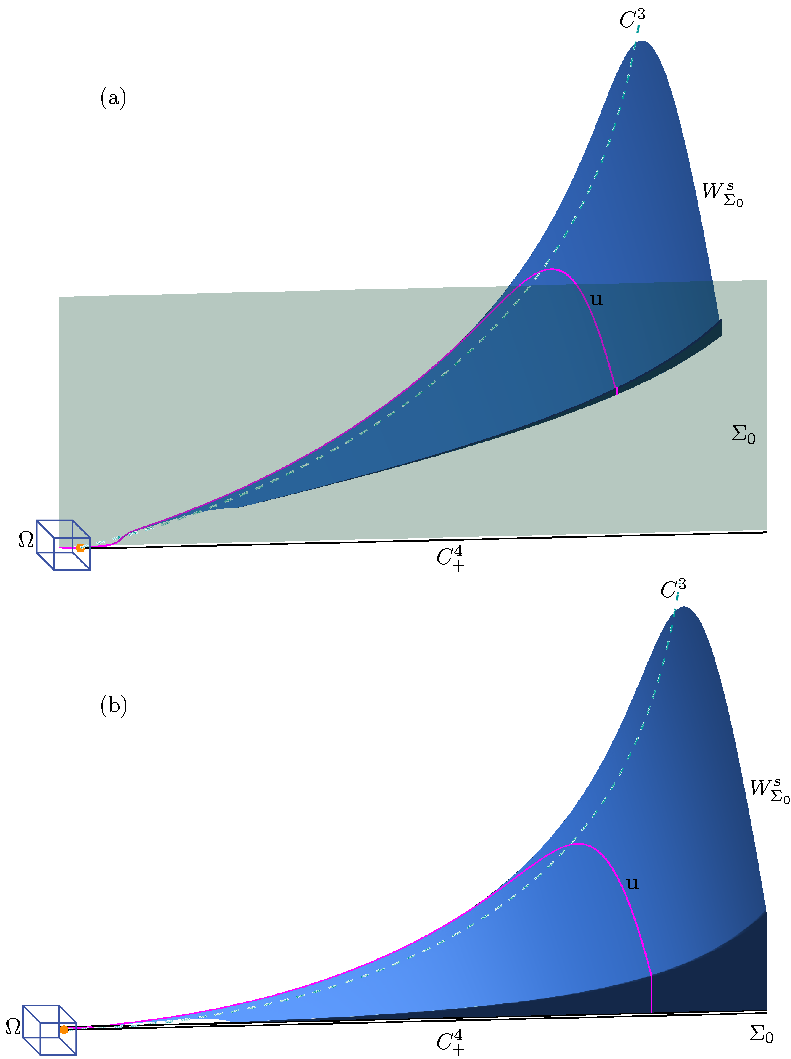
\includegraphics[]{./figures/MKMO_4.pdf}
\caption{The submanifold $W^{s}_{\Sigma_0}$ (light-blue surface) of $W^s(S^3)$, shown in projection into the ($B$, $A$, $X$)-space (a) and into the ($B$, $A$, $Y$)-space (b); also shown are a representative orbit segment $\mathbf{u}$ (magenta curve), the plane $\Sigma_0$ (mint surface and line), $\Omega$ (represented by a blue cube), $C^3$, $C^4_+$, and $F_1$.}
\label{figure_4}
\end{figure}



\begin{figure}[H]
\centering
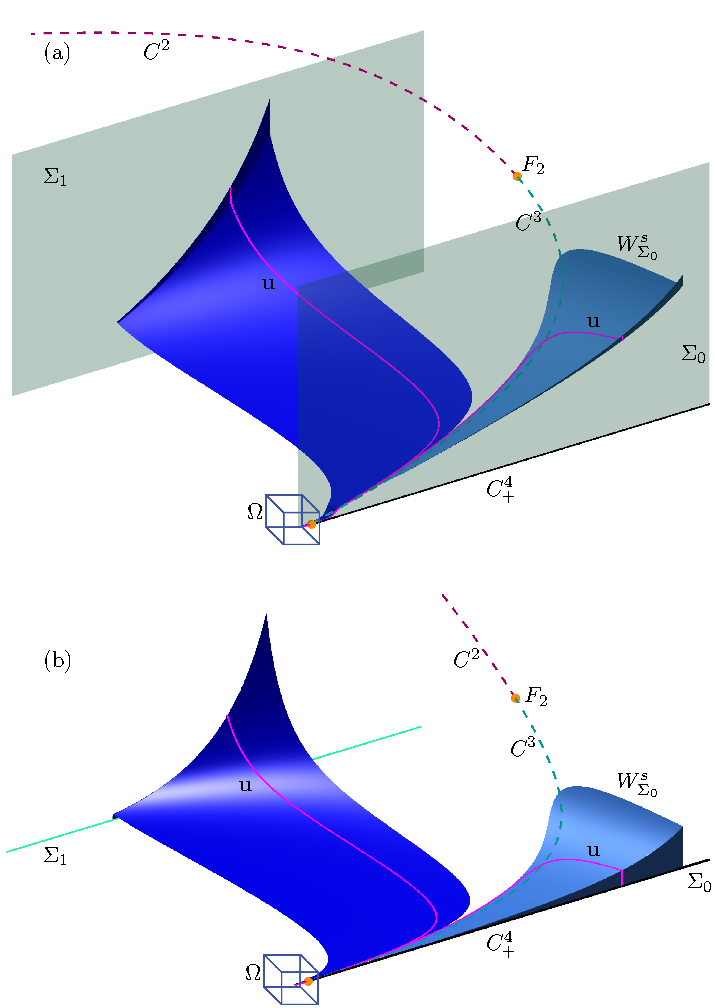
\includegraphics[]{./figures/MKMO_5.pdf}
\caption{The submanifolds $W^{s}_{\Sigma_0}$ (blue surface) and $W^{s}_{\Sigma_0}$ (light-blue surface) of $W^s$, shown in projection into the ($B$, $A$, $X$)-space (a) and into the ($B$, $A$, $Y$)-space (b); also shown are representative orbit segments $\mathbf{u}$ (magenta curves), the planes $\Sigma_0$ (mint surface and line) and $\Sigma_1$ (mint surface and line), and $\Omega$ (represented by a blue cube), $C^2$, $C^3$, $C^4_+$, $F_1$, and $F_2$.}
\label{figure_5}
\end{figure}

Figure \ref{figure_5} shows $W^s_{\Sigma_0}$ (light-blue surface) together with one other submanifold $W^{s}_{\Sigma_1}$ (blue surface) of $W^{s}$ in projection into the ($B$, $A$, $X$)-space (a) and the ($B$, $A$, $Y$)-space (b); here $\Sigma_1$ (mint surface) is given by $A=2.0$ and $Y=0.0$.  The surface $\Sigma_1$ appears as a line in panel (b) because it is defined by constant $A$ and $X$.  The submanifold $W^s_{\Sigma_1}$ is an example of a submanifold on the other side of $C$ with respect to the variable $A$; compare with Figure 3(d).  A representative magenta orbit segment on $W^s_{\Sigma_1}$ is shown approaching $S^3$ first mainly from the $X$- and $Y$-directions, before approaching mostly in the $A$-direction.

\begin{figure}[H]
\centering
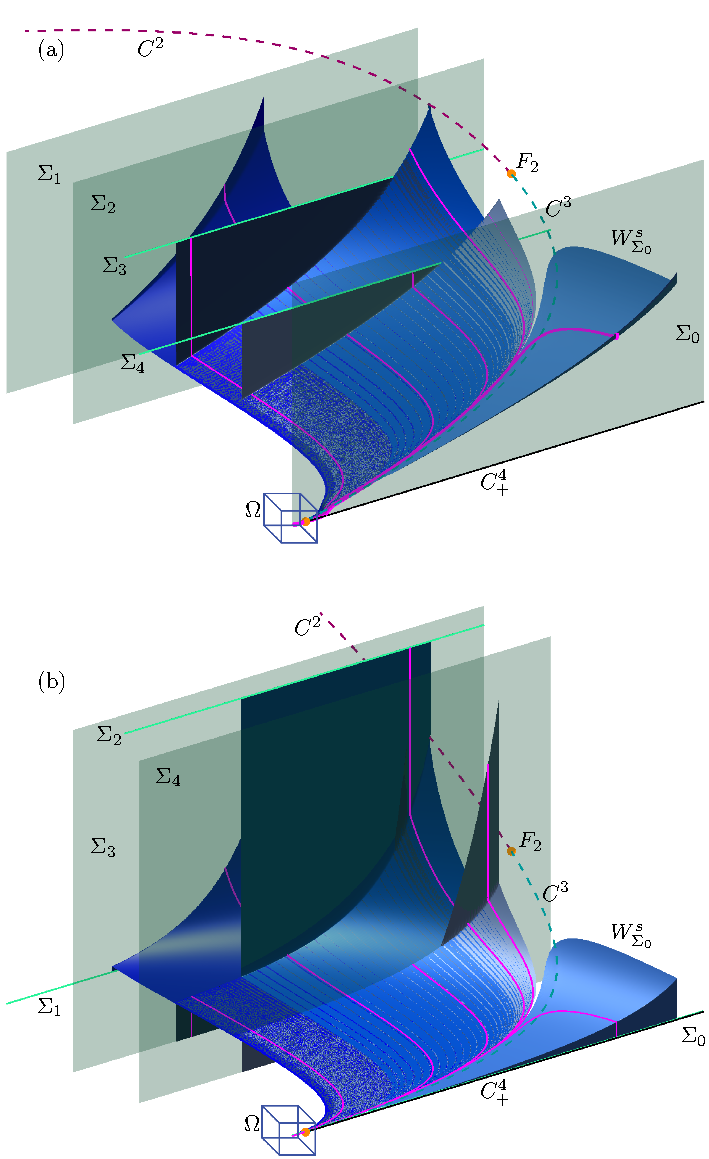
\includegraphics[]{./figures/MKMO_6.pdf}
\caption{The submanifolds from Figure 5 with three additional submanifolds $W^s_{\Sigma_i}$ (blue surfaces) of $W^s$ for $2 \leq i \leq 4$ in projection into the ($B$, $A$, $X$)-space (a) and the ($B$, $A$, $Y$)-space (b); also shown are representative orbit segments $\mathbf{u}$ (magenta curves), the planes $\Sigma_i$ (mint surfaces and lines), and $\Omega$ (represented by a blue cube), $C^2$, $C^3$, $C^4_+$, $F_1$, and $F_2$.}
\label{figure_6}
\end{figure}

Figure \ref{figure_6} shows the two submanifolds of $W^{s}$ from Figure \ref{figure_5} with three additional submanifolds $W^s_{\Sigma_i}$ (blue surfaces), $2 \leq i \leq 4$, and the corresponding planes $\Sigma_i$ (mint surfaces) that define them.  Also shown are $C^3$, $C^4_+$, $F_1$, and $\Omega$.  The additional submanifolds were selected as follows: $\Sigma_2$ is given by $A=4.0$ and $Y=0.75$, $\Sigma_3$ is given by $A=4.0$ and $X=0.75$, and $\Sigma_4$ is given by $A=6.0$ and $X=0.5$.  Note that  $\Sigma_3$ and $\Sigma_4$ appear as lines in panel (a) because they are defined by constant $A$ and $X$.  Similarly, $\Sigma_2$ appears as a line in panel (b) because it is defined by constant values of $A$ and $Y$.  Orbit segments in Figure \ref{figure_6} again first approach $S^3$ in the $X$- and $Y$-directions before approaching in the $A$-direction.  Consequently, there are regions where different submanifolds are extremely close to each other.  In fact, these surfaces are so close that Matlab cannot distinguish them properly.  Different choices of $B_{\text{in}}$ and $B_{\text{out}}$ also cause some submanifolds to extend farther than others in the $B$-direction.

Overall this section and its figures demonstrate that we can reliably compute any number of submanifolds $W^s_\Sigma$ with conditions (\ref{general_conditions_1}),  (\ref{general_conditions_2}), and (\ref{general_conditions_3}) and the homotopy steps outlined above.  Together, these two-dimensional submanifolds provide an understanding of the dynamics inside $W^s(S^3)$.

%unstable
\subsection{Definition and computation of $W^{u}(S^2)$}  

We can define $S^2$ and $W^u(S^2)$ similarly to how we defined $S^3$ and $W^s(S^3)$.  The values for $B_{\text{in}}$ and $B_{\text{out}}$ are chosen such that $[B_{\text{out}}, B_{\text{in}}] \subset (B_q, B_H)$, where $B_q \approx 0.323$ and $B_H \approx 0.897$ are the $B$-values of the saddle equilibrium $q$ and the Hopf point $H$ shown as a green cross and a pink dot, respectively, in Figures \ref{figure_1}, \ref{figure_3}, and \ref{figure_7}. Note that in these figures, the flow near $S^2$ is toward $q$; hence, to the right of $W^u(q)$ the flow is to the left.  Our choice of $B_{\text{out}}>B_{q}$ is to avoid a change in direction of the flow associated with $q$.

To compute a submanifold of $W^{u}(S^2)$ we use slightly different boundary conditions and homotopy steps compared to those used for $W^s(S^3)$ in light of two complicating challenges arising from $q$ and $H$.  Orbit segments near $S^2$ may increase in integration time by approaching $W^s(q)$ or by following the attracting slow manifold associated with $C^4_-$ backwards in time.  We define a submanifold of $W^u(S^2)$ with boundary conditions that ensure that computed orbit segments do not demonstrate these behaviors and only increase in integration time by approaching $S^2$.  

To define $S^2$ and $W^u(S^2)$, we define a three-dimensional cylinder $\mathscr{D}^u$ that is transverse to the flow and to $E^s(C^2)$.  To this end, we choose a radius $r$ and for each $B_p \in [B_{\mathrm{in}}, B_{\mathrm{out}}]$ define the two-dimensional sphere in the subspace $\{\omega \in \mathbb{R}^4 \; | \; B=B_p\}$ centred at $p$ and with radius $r$; here $p \in C^2$ is the unique point such that $p_B = B_p$.  More formally,

\begin{equation*}
D^u_r(B_p)=\{w \in \mathbb{R}^4 \;|\; w_B = B_p, \left\lVert w-p \right\lVert  = r\}.
\end{equation*}
Then 
\begin{equation*}
\mathscr{D}^u = \bigcup\limits_{B_p \in [B_{\mathrm{out}}, B_{\mathrm{in}}]}^{}D^u_r(B),
\end{equation*}
is a three-dimensional cylinder.  We now consider the smooth, one-parameter family of orbit segments of (\ref{equation_1}) is then given by the property that each orbit segment remains inside $\mathscr{D}^u$ for an O(1) amount of slow time, exits $\mathscr{D}^u$ via $D^u_r(B_p)$ for some $B_p \in [B_{\text{out}}, B_{\text{in}}]$ and ends in some plane $\Sigma$.  We denote by $W^u_\Sigma$ those parts of the orbit segments that exit $\mathscr{D}^u$ in the fast direction.  The earlier parts that evolve mostly in the $B$-direction inside $\mathscr{D}^u$ for $O(1)$ slow time are approximate segments of $S^2$.  If such an earlier part of the orbit segment includes a fast entrance into $\mathscr{D}^u$, that fast part lies on $W^s(S^2)$ in good approximation.

We compute the submanifold $W^u_\Sigma$ again as a one-parameter family of orbit segments $\mathbf{w}$ satisfying the rescaled equation (\ref{equation_4}).  Orbit segments $\mathbf{w} \in W^u_\Sigma$ must satisfy the boundary conditions
\begin{equation}
	\mathbf{w}(1) \in \Sigma,
	\label{general_conditions_unstable_1}
\end{equation}

\begin{equation}
	\mathbf{w}(0) \in \Phi = E^u(p_0) \times \begin{bmatrix} 0, 1, 0, 0 \end{bmatrix}^{\prime},
\label{general_conditions_unstable_2}
\end{equation}

\begin{equation}
	\mathbf{w}(0)_B = \widehat{B},
	\label{general_conditions_unstable_3}
\end{equation}
where $p_0 \in C^2$ is such that $p_{0_B} \in (B_{\text{out}}, B_{\text{in}})$ and $\widehat{B}>B_{\text{in}}$.  Equations (\ref{general_conditions_unstable_1}) and (\ref{general_conditions_unstable_2}) are analogous to equations (\ref{general_conditions_1}) and (\ref{general_conditions_2}) from section 3.2.  Equation (\ref{general_conditions_unstable_3}) serves the purpose of preventing $\mathbf{w}$ from increasing in integration time by following the attracting slow manifold associated with $C^4_-$ backward in time; it has no analogue in section 3.2.    Equations (\ref{general_conditions_unstable_1}), (\ref{general_conditions_unstable_2}), and (\ref{general_conditions_unstable_3}) define four conditions on solutions of (\ref{equation_4}) so that there is a well-defined one-parameter family of solutions to this 2PBVP, which represents $W^u_\Sigma$.

Note that the above conditions preclude the selection of $\mathbf{w}$ with maximal integration time as was done in section 3.2 with equation (\ref{general_conditions_3}).  In the case that we would like to impose a condition of maximum integration time, we may substitute for (\ref{general_conditions_unstable_1}) the two conditions
\begin{equation}
	\mathbf{w}(1) \in \mathscr{D}^u,
	\label{general_conditions_unstable_4}
\end{equation}
and
\begin{equation}
	T = T^B,
	\label{general_conditions_unstable_5}
\end{equation}
where for each $B_p \in [B_{\text{out}}, B_{\text{in}}]$, the time $T^B$ is determined as a fold point corresponding to the maximum integration time of an orbit segment that exits $\mathscr{D}^u$ at $B = B_p$ while satisfying (\ref{general_conditions_unstable_2}) and (\ref{general_conditions_unstable_3}).  Indeed, equation (\ref{general_conditions_unstable_4}) imposes one condition on $\mathbf{w}(1)$, one condition less than equation (\ref{general_conditions_unstable_1}), allowing us also to impose equation (\ref{general_conditions_unstable_5}).  Equations (\ref{general_conditions_unstable_2}), (\ref{general_conditions_unstable_3}), (\ref{general_conditions_unstable_4}), and (\ref{general_conditions_unstable_5}) define four conditions on solutions of (\ref{equation_4}) so that there is again a one-parameter family of solutions to this 2PBVP.  We denote the two-dimensional submanifold given by this one-parameter family by $W^u_r$.

Once an initial $\mathbf{w}$ satisfying one of the 2PBVPs  is found, it is possible to sweep out a submanifold $W^u_\Sigma$ or $W^u_r$ by continuing $\mathbf{w}$ with varying $\mathbf{w}(1)_B$ and $T_B$.  The challenge is, once again, the computation via homotopy steps of an initial orbit segment satisfying the boundary conditions.

In the first homotopy step, we choose the point $p_0=\begin{pmatrix} p_{0_A}, p_{0_B}, p_{0_X}, p_{0_Y} \end{pmatrix} \in C^2$ by fixing $p_{0_B}=B_0 \in [B_{\text{out}}, B_{\text{in}}]$.  We impose condition (\ref{general_conditions_unstable_2}) as well as the condition
	\begin{equation}
		\mathbf{w}(1) \in \chi = \{ \omega \in \mathbb{R}^4 \; | \; \omega_A=p_{0_A}, \omega_B=p_{0_B} \omega_Y=p_{0_Y} \}.
		\label{specific_BC_unstable1}
	\end{equation}
The point $p_0$ is then a solution to (\ref{general_conditions_unstable_2}) and (\ref{specific_BC_unstable1}) for $T=0$.  We increase $\mathbf{w}_B$ with $T$ as a free parameter and stop the continuation when $\mathbf{w}_B=\widehat{B}$.  The value of $\mathbf{w}_B$ is fixed from this step onwards.  We define the two-dimensional space

\begin{equation*}
	\Phi_{\widehat{B}} = \Phi \cap \{ \omega \in \mathbb{R} \; | \; \omega_B=\widehat{B}\}.
\end{equation*}

In the second homotopy step, we substitute equation (\ref{specific_BC_unstable1}) for (\ref{general_conditions_unstable_1}) with $\Sigma=\{ \omega \in \mathbb{R}^4 \;|\; \omega_A=p_{0_A}, \omega_Y=p_{0_Y} \}$ and impose (\ref{general_conditions_unstable_3}).  The orbit segment $\mathbf{w}$ at the end of the first homotopy step is then a solution to this 2PBVP defined by (\ref{equation_4}), (\ref{general_conditions_unstable_1}), (\ref{general_conditions_unstable_2}), and (\ref{general_conditions_unstable_3}).  It is in this second homotopy step that we decide whether to compute a submanifold $W^u_\Sigma$ or $W^u_r$.  If our aim is to compute $W^u_\Sigma$, all that remains to compute an initial $\mathbf{w}$ lying on the manifold is to move $\Sigma$ to a desired location as in section 3.2.  To compute $W^u_r$ we increase $T$ until $\mathbf{w}(1) \in \Sigma \cap \mathscr{D}^u$.  This is detected as $\mathbf{w}(1)$ reaching a distance of $r$ away from the point $p \in C^2$ such that $p_B = \mathbf{w}_B$.  We denote the coordinates $\mathbf{w}(1)_B$ and $\mathbf{w}(1)_X$ of the end point at the end of this step by $\widetilde{B}$ and $\widetilde{X}$, respectively.  

In the event that $D_r(\widetilde{B})$ contains a locus of points at which the flow is tangent to it, we perform a third homotopy step to increase $\widetilde{B}$ until the flow is transverse to $D_r(\widetilde{B})$.  This is achieved by imposing conditions (\ref{general_conditions_unstable_2}), (\ref{general_conditions_unstable_3}), and (\ref{general_conditions_unstable_4}) on $\mathbf{w}$ at the end of the second homotopy step and then increasing $\mathbf{w}_B$ while keeping $T$ as a free parameter.

In the final homotopy step, we replace condition (\ref{general_conditions_unstable_4}) with 
	\begin{equation}
		\mathbf{w}(1) \in \Theta = D^u_r(\widetilde{B}) \cap \{ \omega \in \mathbb{R} \; | \; \omega_X = \widetilde{X} \}.
		\label{specific_BC_unstable2}
	\end{equation}
The orbit segment $\mathbf{w}$ at the end of the second homotopy step (or the third homotopy step if one was necessary) is then a solution to the 2PBVP defined by (\ref{equation_4}), (\ref{general_conditions_unstable_2}), (\ref{general_conditions_unstable_3}), and (\ref{specific_BC_unstable2}).    We now increase $T$ until $T=T^B$, which is detected as a fold in integration time.  The resulting orbit segment $\mathbf{w}$ lies on $W^u_r$.

Once an initial orbit segment $\mathbf{w}$ on either $W^u_\Sigma$ or $W^u_r$ is found, we may sweep out the remaining part of the submanifold by increasing and decreasing $\mathbf{w}_B$ and keeping $T^B$ as a free parameter so that it can be adjusted accordingly for the fold detection.

Figure \ref{figure_7} illustrates, in projection onto the $(B,A)$-plane, the adjusted homotopy steps for computing $W^u_r$.  Each panel shows an enlargement of the critical manifold $C$ from Figure \ref{figure_1} near $C^2$ with additional information for the computation.   We choose $p_0=\begin{pmatrix} 0.940272, && 0.7, && 1.492271, && 1.342954 \end{pmatrix}$ which lies approximately on $C^2$.  In the first homotopy step, we impose condition (\ref{specific_BC_unstable1}), which imposes three conditions on $\mathbf{w}(1)$, as well as condition (\ref{general_conditions_unstable_2}), which imposes one restriction on $\mathbf{w}(0)$.  Panel (a) shows a sketch of an intermediate situation in the first homotopy step; here, we show $\mathbf{w}$ (forest green curve), the one-dimensional line $\chi$ sketched in mint, and the three-dimensional $\Phi$ sketched as a mint prism.  The $B$-coordinate of $\mathbf{w}(0)$ is increased with $T$ as a free parameter.  The continuation is stopped when $\mathbf{w}(0)_B=\widehat{B}$ for $\widehat{B}=1.0$.  In the second homotopy step, we impose (\ref{general_conditions_unstable_1}), (\ref{general_conditions_unstable_2}), and (\ref{general_conditions_unstable_3}), increasing $\mathbf{w}(1)_B$ with $T$ as a free parameter until $\mathbf{w}(1)$ intersects $\mathscr{D}^u$ for $r=0.7$.  We are not required to perform an additional homotopy step because $D_r(\widetilde{B})$, in this case, does not contain a locus of points at which the flow is tangent to it.  Figure \ref{figure_7}(b) shows a sketch of the numerical set up before the final homotopy step; here, the one-dimensional closed curve $\Theta$ is sketched in mint and $\Phi_{\widehat{B}}$ is sketched as a mint cross. We then impose (\ref{general_conditions_unstable_2}), (\ref{general_conditions_unstable_3}), (\ref{general_conditions_unstable_4}) and (\ref{general_conditions_unstable_5}) and increase $T$.  The continuation is stopped when $T=T^B$ which is again detected as a fold.  The resulting orbit segment lies on $W^u_r$.  We can then sweep out the rest of the submanifold $W^u_r$ by continuing the fold in integration time for increasing and decreasing $\mathbf{w}(1)_B$.

\begin{figure}[H]
\centering
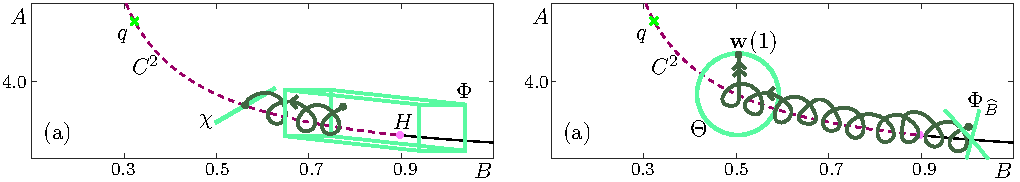
\includegraphics[]{./figures/MKMO_7.pdf}
\caption{A sketch in projection onto the ($B$,$A$)-plane of the homotopy steps for the computation of submanifolds $W^u_r$ of $W^u(S^2)$.  Also shown are $C^2$ (dashed raspberry curve), $C^4_-$ (black curve), $H$ (pink dot), $q$ (green cross), and the orbit segment $\mathbf{w}$ (forest green curve).  Panel (a) is a sketch of the situation during the first homotopy step with $\chi$ (mint line) and $\Phi$ (mint prism); panel (b) is a sketch of the start of the final homotopy step with $\Theta$ (mint circle) and $\Phi_{\widehat{B}}$ (mint cross).}
\label{figure_7}
\end{figure} 

\begin{figure}[H]
\centering
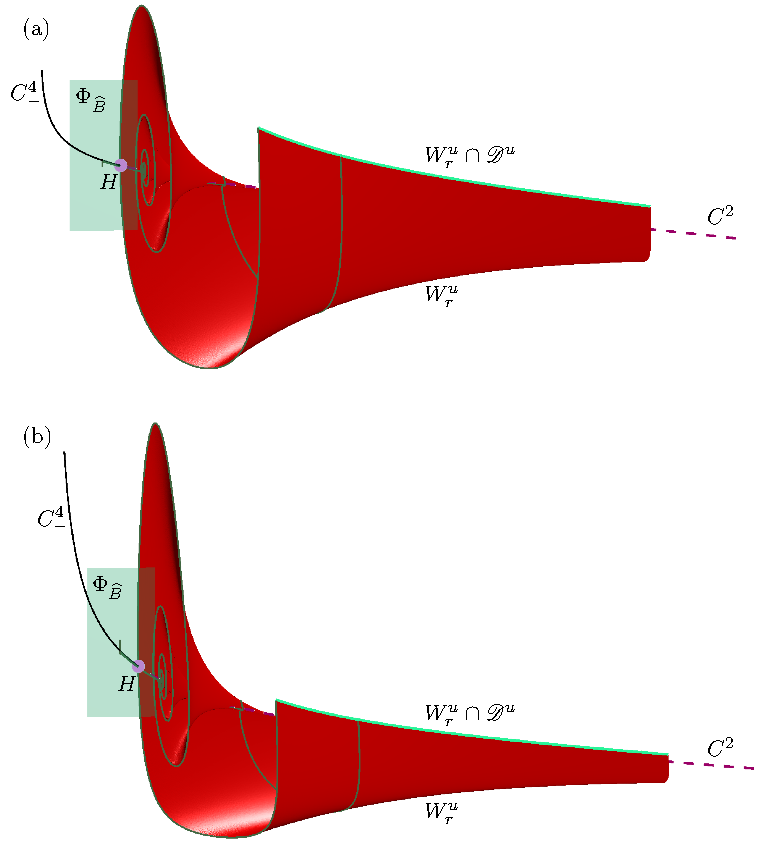
\includegraphics[]{./figures/MKMO_8.pdf}
\caption{The submanifold $W^u_{r}$ (red surface) of $W^u(S^2)$ for $r=0.7$ shown in projection onto $(B,A,X)$-space (a) and $(B,A,Y)$-space (b); note that the view is rotated compared to previous figures.  Also shown are two representative orbit segments $\mathbf{w}$ (forest green curves) on $W^u_{r}$, the two-dimensional space $\Phi_{\widehat{B}}$ (mint surface), the one-dimensional intersection $W^s_{r}\cap\mathscr{D}^u$ (mint curve), along with the curves $C^2$ and $C^4_-$, and the point $H$.}
\label{figure_8}
\end{figure}

Figure \ref{figure_8} shows two projections of the submanifold $W^u_{r}$ for $r=0.7$ with $W^u_{r} \cap \mathscr{D}^u$ (mint curve) and $\Phi_{\widehat{B}}$ (mint surface).  Note that $W^u_{r}\cap\mathscr{D}^u$ is simply the curve traced out by $\mathbf{w}(1)$.  To facilitate viewing, the view is rotated compared to previous figures.  Two representative orbit segments $\mathbf{w}$ are plotted and a subset of $C^2$ (dashed raspberry curve) is shown.  From this angle, the radius of $\mathscr{D}^u$ may, to some readers, appear to decrease with decreasing $\mathbf{w}(1)_B$.  This is due to the eye's erroneous association of points $\mathbf{w}(1)$ with points $p \in C^2$ such that $p_B < \mathbf{w}(1)_B$.  Due to the spiralling nature of $W^u_r$, we only show one such submanifold for ease of visualization.

%Lin's method

\section{A heteroclinic connection between two saddle slow manifolds}

\begin{figure}[H]
\centering
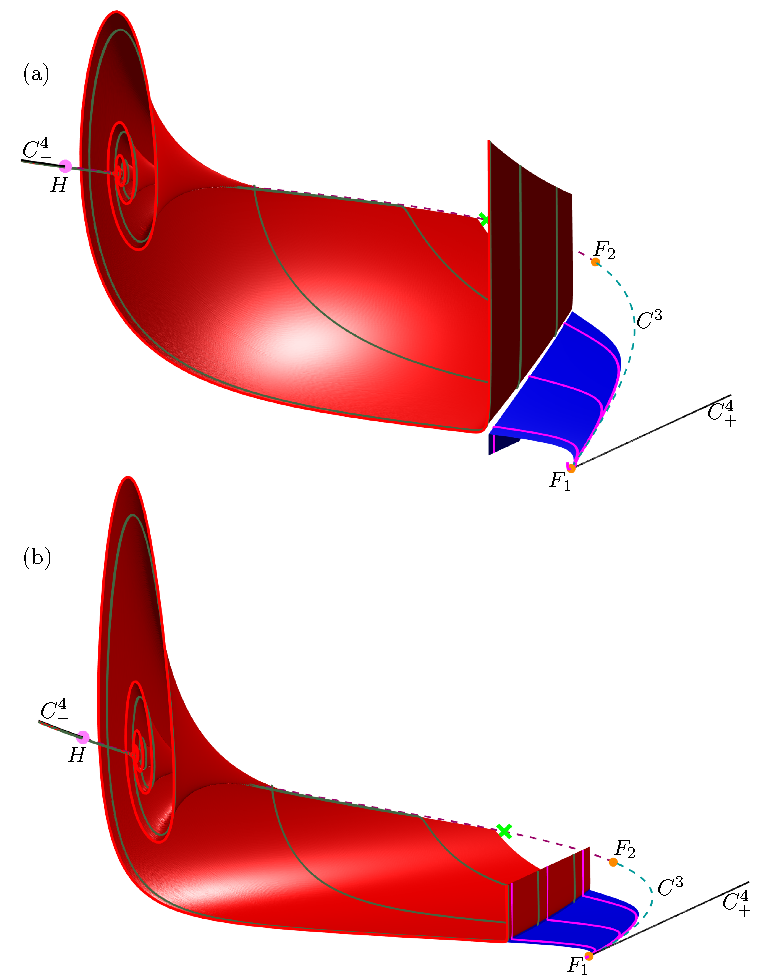
\includegraphics[]{./figures/MKMO_9.pdf}
\caption{The submanifold $W^u_{\Sigma_5}$ (red surface) of $W^u(S^2)$ and the submanifold $W^s_{\Sigma_5}$ (blue surface) of $W^s(S^3)$ in projection onto $(B,A,X)$-space (a) and onto $(B,A,Y)$-space (b). Representative orbit segments $\mathbf{w} \in W^u_{\Sigma_5}$ and $\mathbf{u} \in W^u_{\Sigma_5}$ are plotted in forest green and magenta, respectively; also shown are $C^2$, $C^3$, $C^4_\pm$, $F_1$, $F_2$, $H$, and $q$ (which is partially obscured by the two-dimensional submanifold $W^u_{\Sigma_5}$). }
\label{figure_9}
\end{figure}

Two three-dimensional objects in a four-dimensional space may intersect generically in a two-dimensional manifold.  It follows, then, that the three-dimensional $W^s(S^3)$ and the three-dimensional $W^u(S^2)$ may intersect in a two-dimensional surface of heteroclinic connections which we denote $\mathscr{H}$.  This is supported by the fact that, for the reduced system in \cite{QSSA}, there exists a two-dimensional stable manifold associated with the branch equivalent to $C^3$ that stretches backward in time all the way to the branch equivalent to $C^2$.  Hence, we wish to detect and compute a surface of connections which we denote $\mathscr{H}$.  A natural way forward is to consider $\mathscr{H}$ as a one-parameter family of concatenations of orbit segments $\mathbf{w} \in W^u(S^2)$ with $\mathbf{u} \in W^u(S^3)$.

A first idea is to compute two two-dimensional submanifolds $W^u_\Sigma$ and $W^s_\Sigma$ up to a suitable choice of a single two-dimensional section $\Sigma$.  However, these two two-dimensional objects do not generically intersect in a four-dimensional space.  Figure \ref{figure_9} demonstrates this difficulty.  The chosen section $\Sigma_5=\{\omega \in \mathbb{R}^4 \;|\; \omega_A= 6.0, \omega_Y=0.5 \}$ yields the submanifolds $W^s_{\Sigma_5}$ (blue surface) and $W^u_{\Sigma_5}$ (red surface) shown in Figure \ref{figure_9}.  Representative orbit segments $\mathbf{w}$ (forest green curves) and $\mathbf{u}$ (magenta curves) are shown coming toward each other mostly in the $A$-direction before diverging away from each other in the faster $X$- and $Y$-directions.  Although the submanifolds appear to intersect in the ($B$, $A$, $Y$)-projection in Figure \ref{figure_9}(b), we can see from the ($B$, $A$, $X$)-projection in Figure \ref{figure_9}(a) that the $W^s_{\Sigma_5}$ and $W^u_{\Sigma_5}$, in fact, miss each other in the four-dimensional phase space.  Nevertheless, we are encouraged by the closeness of $W^u_{\Sigma_5}$ and $W^s_{\Sigma_5}$, which suggests that a nearby surface $\mathscr{H}$ of connecting orbits could exist.

We turn to Lin's method to find the actual surface of connecting orbits $\mathscr{H}$.  Lin's method has been used in parameter continuation to locate connections between equilibria and/or periodic orbits \cite{Lin_original, Lin_POs, Lin_POs2}.  We use it here in a novel way to locate structurally stable connections between $S^2$ and $S^3$ for the system parameters given in the four-dimensional space of system (\ref{equation_1}).

We begin by choosing a three-dimensional section $\mathscr{L}$, called a Lin section, that divides the four-dimensional phase space into two regions such that $C^3$ lies in one region and $C^2$ lies in the other.  More specifically, the Lin section $\mathscr{L}$ is defined by a constant value of $A$ that is chosen so that $\mathscr{L}$ intersects $C$ to the left of $W^u(q)$ in the ($B$, $A$)-projection; this choice of $\mathscr{L}$ allows us to compute the largest possible portion of $\mathscr{H}$ to the right of $W^u(q)$.  Inside $\mathscr{L}$ we choose a unit vector $\mathbf{v}_Z$ with the generic property that it is not tangent to either $W^u(S^2)$ or $W^s(S^3)$.  The vector $\mathbf{v}_Z$ is called a Lin vector and the space $Z$ spanned by $\mathbf{v}_Z$ the associated Lin space.  We then use the methods outlined in section 3 to compute $\mathbf{u} \in W^s(S^3)$ and $\mathbf{w} \in W^u(S^2)$ such that
\begin{equation}
	\mathbf{u}(0) \in \mathscr{L}
	\label{general_conditions_heteroclinic_1}
\end{equation}
and
\begin{equation}	
	 \mathbf{w}(1) \in \mathscr{L}.
	 \label{general_conditions_heteroclinic_2}
\end{equation}
Additionally, we require that
\begin{equation*}
	\mathbf{u}(0)-\mathbf{w}(1) \in Z.
\end{equation*}
Note that the difference $\mathbf{u}(0)-\mathbf{w}(1)$ or arbitrary orbit segments $\mathbf{u} \in W^s(S^3)$ and $\mathbf{w} \in W^u(S^2)$ will typically correspond to a vector direction $\mathbf{v}_Z$ that is transverse to both manifolds.  Hence, effectively we first compute two orbit segments $\mathbf{u}$ and $\mathbf{w}$ on the respective manifolds and then decide on the choice for $\mathbf{v}_Z$.  Importantly, the signed distance between $\mathbf{u}(0)$ and $\mathbf{w}(1)$ inside $Z$, given by
\begin{equation}
	\eta=[\mathbf{u}(0)-\mathbf{w}(1)] \cdot \mathbf{v}_Z,
	\label{general_conditions_heteroclinic_3}
\end{equation}
is a regular test function.  Note that $\left\lvert \eta \right\lvert = \left\lVert \mathbf{u}(0)-\mathbf{w}(1) \right\lVert$.  A pair of orbit segments ($\mathbf{w}$, $\mathbf{u}$) with 
\begin{equation}
	\eta = 0
	\label{general_conditions_heteroclinic_4}
\end{equation}
is then a connection between $S^2$ and $S^3$.  Hence, finding a zero of $\eta$ is the way of finding a connecting orbit in $\mathscr{H}$.

To implement $\mathbf{u}(0), \mathbf{w}(1) \in Z$, we define unit normal vectors $\mathbf{n}_1 \perp \mathbf{v}_Z$ and $\mathbf{n}_2 \perp \mathbf{v}_Z$ in $\mathscr{L}$ such that $\mathbf{n}_1 \perp \mathbf{n}_2$ and impose conditions

\begin{equation}
	[\mathbf{u}(0) - \mathbf{w}(1)] \cdot \mathbf{n}_1 =0
	\label{general_conditions_heteroclinic_5}
\end{equation}
and
\begin{equation}	
	 [\mathbf{u}(0) - \mathbf{w}(1)] \cdot \mathbf{n}_2 =0.
	 \label{general_conditions_heteroclinic_6}
\end{equation}
Equations (\ref{general_conditions_heteroclinic_5}) and (\ref{general_conditions_heteroclinic_6}) ensure that $\mathbf{w}(1)-\mathbf{u}(0)$ remains in $Z$.  Conditions (\ref{general_conditions_heteroclinic_3}) and (\ref{general_conditions_heteroclinic_4}) together ensure that $\mathbf{w}(1) = \mathbf{u}(0)$.  Once an initial pair of orbit segments $(\mathbf{w}, \mathbf{u})$ satisfying the above conditions is found, the surface $\mathscr{H}$ can be swept out, for example by varying $\mathbf{w}(1)_B$ with $\mathbf{u}(0)_B$ and $T$ as additional free parameters.  

The challenge is, as always, to find an initial pair $(\mathbf{w}, \mathbf{u})$ satisfying the required BCs via a series of homotopy steps.  In the first homotopy step we compute $\mathbf{w} \in W^u_{\Sigma_{L_1}}$ and $\mathbf{u} \in W^s_{\Sigma_{L_2}}$ for $\Sigma_{L_1} $, $\Sigma_{L_2} \subset \mathscr{L}$, requiring (\ref{general_conditions_1}) and (\ref{specific_BC}) for $\mathbf{u}$ and (\ref{general_conditions_unstable_1}), (\ref{general_conditions_unstable_2}), and (\ref{general_conditions_unstable_3}) for $\mathbf{w}$.  In particular, (\ref{general_conditions_heteroclinic_1}) and (\ref{general_conditions_heteroclinic_2}) are then satisfied and we choose
	\begin{equation*}
		\mathbf{v}_Z = \frac{\mathbf{u}(0) - \mathbf{w}(1)}{\left\lVert \mathbf{u}(0) - \mathbf{w}(1) \right\lVert},
		\label{Lin_vector}
	\end{equation*}
which is a convenient choice of a vector that is (generically) transverse to $W^u(S^2)$ and $W^s(S^3)$. We then find the vectors $\mathbf{n}_1$ and $\mathbf{n}_2$ required for conditions (\ref{general_conditions_heteroclinic_1}) and  (\ref{general_conditions_heteroclinic_2}). Once chosen, the vector $\mathbf{v}_Z$ and normal vectors $\mathbf{n}_1$ and $\mathbf{n}_2$ remains fixed throughout the computations.

The conditions imposed in the first homotopy step define a two-parameter family of paired orbit segments ($\mathbf{w}$, $\mathbf{u}$) that meet in $\mathscr{L}$ along $Z$.  In the second homotopy step, we now relax conditions (\ref{general_conditions_1}) and (\ref{general_conditions_unstable_1}), which respectively are two conditions each on $\mathbf{u}$ and $\mathbf{w}$, and impose instead conditions (\ref{general_conditions_heteroclinic_1}) and (\ref{general_conditions_heteroclinic_2}), (\ref{general_conditions_heteroclinic_3}), (\ref{general_conditions_heteroclinic_5}) and (\ref{general_conditions_heteroclinic_6}).    Conditions (\ref{general_conditions_heteroclinic_1}) and  (\ref{general_conditions_heteroclinic_2}), impose one condition on $\mathbf{u}$ and one condition on $\mathbf{w}$, respectively.  Conditions  (\ref{general_conditions_heteroclinic_5}) and (\ref{general_conditions_heteroclinic_6}) impose two conditions on ($\mathbf{w}$, $\mathbf{u}$).  The number of boundary conditions imposed is, hence, the same as in the first homotopy step, and thus, they define a two-parameter family of paired orbit segments ($\mathbf{w}$, $\mathbf{u}$).  To choose a one-parameter family ($\mathbf{w}$,$\mathbf{u}$) from these, we impose the additional boundary condition 
	\begin{equation}
		\mathbf{w}(1)_B = B_1,
		\label{specific_BC_hetclin}
	\end{equation}
where $B_1$ is the value of the $B$-coordinate of $\mathbf{w}(1)$ at the end of the first homotopy step.  We now continue $(\mathbf{w}, \mathbf{u})$ as a solution to the 2PBVP defined by (\ref{specific_BC}), (\ref{general_conditions_unstable_2}), (\ref{general_conditions_heteroclinic_1}) and (\ref{general_conditions_heteroclinic_2}), (\ref{general_conditions_heteroclinic_3}) and (\ref{general_conditions_heteroclinic_5}), (\ref{general_conditions_heteroclinic_6}), and (\ref{specific_BC_hetclin}) with $T$ and $\mathbf{u}(0)_B$ as free parameters.  We monitor condition (\ref{general_conditions_heteroclinic_3}) and stop the continuation when $\eta=0$, at which point condition (\ref{general_conditions_heteroclinic_4}) is satisfied and the concatenation of $\mathbf{w}$ with $\mathbf{u}$ is a connecting orbit segment in $\mathscr{H}$.  We can then sweep out the portion of $\mathscr{H}$ to the right of $W^u(q)$ in the ($B$, $A$)-projection by replacing condition (\ref{specific_BC_hetclin}) with (\ref{general_conditions_heteroclinic_4}), and allowing $\mathbf{u}(0)_B$, $\mathbf{w}(1)_B$ to vary again.

Figure \ref{figure_10} illustrates, step-by-step in projection onto the ($B$, $A$)-plane, the homotopy steps for computing the portion of $\mathscr{H}$ to the right of $W^u(q)$.  
Each panel shows $C$ from Figure \ref{figure_1} with $\mathscr{L} = \{ \omega \in \mathbb{R}^4 \; | \; \omega_A = 6.0 \}$ (charcoal line), $\mathbf{u} \in W^s_{\Sigma_{L_1}}$ (magenta curve), $\mathbf{w} \in W^u_{\Sigma_{L_2}}$ (forest green curve), the stable eigenspace $E^s(p_{\text{out}})$ (blue cross) from condition (\ref{specific_BC}), the two-dimensional space $\Phi_{\widehat{B}}$ (mint cross) from conditions (\ref{general_conditions_unstable_2}) and (\ref{general_conditions_unstable_3}).  
In the first homotopy step, we choose $\Sigma_{L_1}=\{ \omega \in \mathbb{R}^4 \; | \; \omega_A = 6.0, \omega_Y=-1.0 \}$ and $\Sigma_{L_2}=\{ \omega \in \mathbb{R}^4 \; | \; \omega_A = 6.0, \omega_Y=3.0 \}$.  We compute $\mathbf{w}$ so that $\mathbf{w}(1)_B = B_1 = 0.6$ in the second homotopy step.  Figure \ref{figure_10}(a) is a sketch of the numerical set-up at the end of the first homotopy step.  The points $\mathbf{w}(1)$ and $\mathbf{u}(0)$ lie in the space $Z$ (gold line) from conditions (\ref{general_conditions_heteroclinic_5}) and (\ref{general_conditions_heteroclinic_6}) at a distance $\eta$ from each other.  Panel (b) is a sketch of the numerical set-up after the second homotopy step when $\mathbf{w}(1) = \mathbf{u}(0)$ and $\eta=0$.  The resulting pair ($\mathbf{w}$, $\mathbf{u}$) satisfies conditions (\ref{general_conditions_heteroclinic_1}) and (\ref{general_conditions_heteroclinic_2})--(\ref{general_conditions_heteroclinic_4}) and their concatenation lies on the surface $\mathscr{H}$.


\begin{figure}[H]
\centering
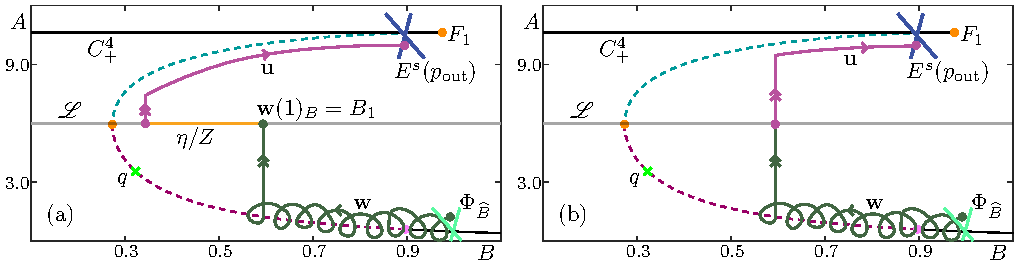
\includegraphics[]{./figures/MKMO_10.pdf}
\caption{A sketch in projection onto the ($B$,$A$)-plane of the numerical set-up with Lin's method for the computation of $\mathscr{H}$ to the right of $W^u(q)$.  Also shown are $C^2$, $C^3$, $C^4_\pm$, $F_1$, $F_2$, $H$, and $q$.  Panel (a) shows a sketch at the end of the first homotopy step with $\mathbf{u} \in W^u_{L_1}$ (magenta curve)$, \mathbf{w} \in W^u_{L_2}$ (forest green curve), $\Phi_{\widehat{B}}$ from section 3.2, and the Lin space $Z$ (gold line) in which the points $\mathbf{w}(1)$ and $\mathbf{u}(0)$ lie at a distance $\eta$ from each other.  Panel (b) shows $\mathbf{w}$ and $\mathbf{u}$ after the final homotopy step at which point $\eta=0$ and $\mathbf{w}(1)=\mathbf{u}(0)$.}
\label{figure_10}
\end{figure}

After these homotopy steps, we use boundary conditions (\ref{general_conditions_heteroclinic_1}) and (\ref{general_conditions_heteroclinic_2}), (\ref{general_conditions_heteroclinic_3}), (\ref{general_conditions_heteroclinic_4}), and (\ref{general_conditions_heteroclinic_5}) and (\ref{general_conditions_heteroclinic_6}) to sweep out a one-parameter family of paired orbit segments to obtain an accurate approximation of $\mathscr{H}$ to the right of $W^u(q)$.  Figure \ref{figure_11} shows the computed portion of $\mathscr{H}$ (red/blue surface) with $\mathscr{L}$ (charcoal plane) in projection onto ($B$, $A$, $X$)-space (a) and ($B$, $A$, $Y$)-space (b).  Three concatenated orbit segments ($\mathbf{w}$, $\mathbf{u}$) lying on $\mathscr{H}$ are plotted in forest green for $\mathbf{w}$ and magenta for $\mathbf{u}$.  The portion of the surface swept out by $\mathbf{w}$ is shown in red and that by $\mathbf{u}$ in blue.  Unlike other manifolds $W^s_\Sigma$ and $W^u_\Sigma$, the paired orbit segments ($\mathbf{w}$, $\mathbf{u}$) on $\mathscr{H}$ do not contain segments that diverge quickly in the directions parallel to the $X$- and $Y$-axes.  Orbit segments lying on $\mathscr{H}$ spiral slowly around $S^2$ before crossing the surface at an intermediate speed, mostly in the direction parallel to the $A$-axis, to reach and then slowly follow $S^3$.

Figure \ref{figure_12} shows that the computed portion of $\mathscr{H}$ is bounded by $W^u(q)$ (cardinal surface; this surface was computed with the BVP approach outlined in \cite{Red_book}).  Here $\mathscr{H}$ is colored red near $S^2$ and blue near $S^3$ to illustrate that $\mathscr{H}$ is both a submanifold of $W^u(S^2)$ and of $W^s(S^3)$; compare with Figure \ref{figure_11}.  Similarly, concatenated orbit segments ($\mathbf{w}$, $\mathbf{u}$) are plotted fading from forest green to magenta.  Orbits on $\mathscr{H}$ clearly follow $S^2$ on the slow time-scale, before traversing across $\mathscr{H}$ on an intermediate time-scale and then following $S^3$ on the slow time-scale.  As this figure shows, the saddle point $q$ and its two-dimensional unstable manifold $W^u(q)$ bound the computed portion of $\mathscr{H}$.  Notice how the connecting orbits nearest $W^u(q)$ follow this two-dimensional surface to come very close to $q$, before slowly following $S^2$. Hence, we computed the part of $\mathscr{H}$ to this side of $q$ as closely to $W^u(q)$ as possible.

\begin{figure}[H]
\centering
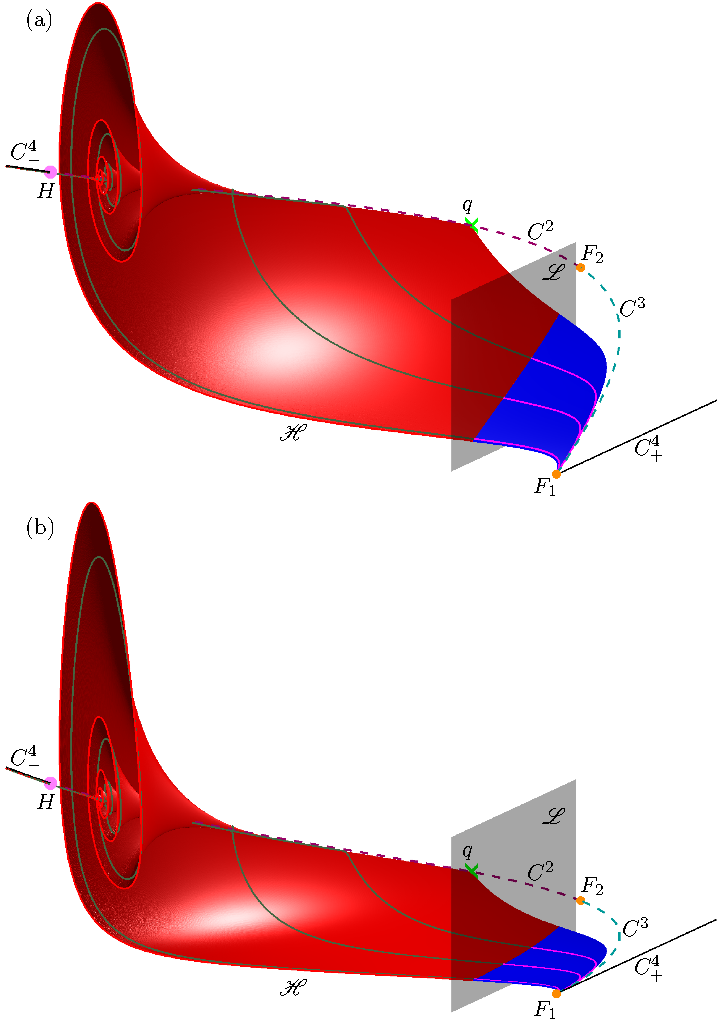
\includegraphics[]{./figures/MKMO_11.pdf}
\caption{The surface of heteroclinic connections $\mathscr{H}$ (red/blue surface) and the Lin section $\mathscr{L}$ (charcoal surface) in projection onto $(B,A,X)$-space (a) and onto $(B,A,Y)$-space (b).  The portion of $W^u(S^2)$ swept out by the family of $\mathbf{w}$ is colored red and the portion of $W^s(S^3)$ swept out by the family of $\mathbf{u}$ blue.  Also shown are representative concatenated orbit segments ($\mathbf{w}$,$\mathbf{u}$) (forest green/magenta curves), the curves $C^2$, $C^3$, and $C^4_\pm$, and the points $F_1$, $F_2$, $H$ and $q$ which is partially obscured by $\mathscr{H}$ and $\mathscr{L}$.}
\label{figure_11}
\end{figure}

\begin{figure}[H]
\centering
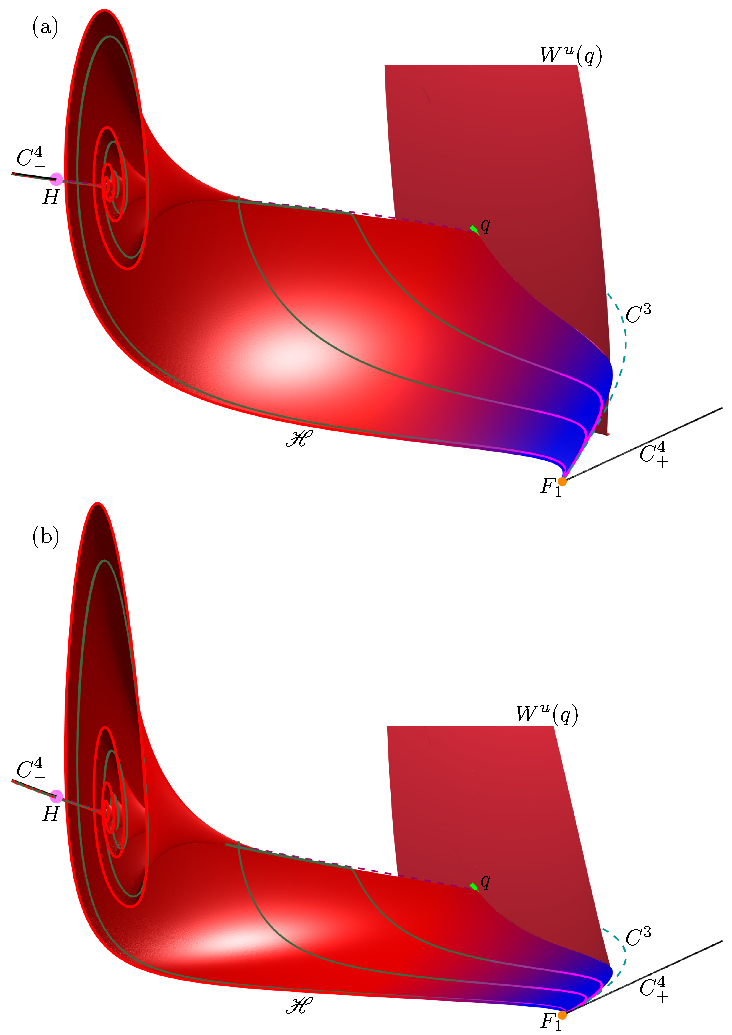
\includegraphics[]{./figures/MKMO_12.pdf}
\caption{The computed portion of $\mathscr{H}$ (red-blue fade surface) is shown in projection onto $(B,A,X)$-space (a) and onto $(B,A,Y)$-space (b) with $W^u(q)$ (cardinal surface).  The unstable manifold $W^u(q)$ bounds the computed portion of $\mathscr{H}$.  Also shown are representative concatenated orbit segments ($\mathbf{w}$, $\mathbf{u}$) (forest green-magenta fade curves), the curves $C^2$, $C^3$, and $C^4_\pm$, and the points $F_1$, $F_2$, $H$ and $q$ which is partially obscured by $\mathscr{H}$ and $W^u(q)$.}
\label{figure_12}
\end{figure}
%%%%%%%%singular limit surface
\section{Computing the surface of heteroclinic connections in the singular limit}

We now consider the limiting surface $\mathscr{H}_0$ of connecting orbits from $C^2$ to $C^3$ for $\varepsilon = 0$.  Recall that system (\ref{equation_1}) then reduces to the three-dimensional system (\ref{equation_2}) in which $B$ is a parameter.  Hence, the surface $\mathscr{H}_0$ is the one-parameter family, parametrized by $B$, of connections between the saddle equilibria of (\ref{equation_2}) on $C^2$ and on $C^3$, respectively.  It is simple to sweep out $\mathscr{H}_0$ with varying $B$ once an initial connection is found for fixed $B$.  The problem then reduces to finding a heteroclinic connection between two saddle equilibria in a three-dimensional system.  This is exactly the situation addressed in \cite{Lin,Red_book} and we now briefly explain how this approach can be used for our purposes.

Note that we now rescale system (\ref{equation_2}), that is, we consider
\begin{equation}
\frac{d\mathbf{u}}{ds} = TG(\mathbf{u}),
\label{fast_rescale}
\end{equation}
where $\mathbf{u}(s) = (A(s), X(s), Y(s)) \in \mathbb{R}^3$ is now a three-dimensional vector, $G$ is the right-hand side of (\ref{equation_2}), and $T$ is the integration time on the fast time-scale.

We compute $\mathscr{H}_0$ as the one parameter family of concatenated orbit segments ($\mathbf{w}$, $\mathbf{u}$), that are solutions of (\ref{fast_rescale}).  We again turn to Lin's method to find an initial orbit segment pair lying on $\mathscr{H}_0$ via homotopy steps.  We begin by choosing a $\widehat{B} \in (B_{\text{in}}, B_{\text{out}})$ corresponding to points $\widehat{p}^2 \in C^2$ and $\widehat{p}^3 \in C^3$.  A two-dimensional Lin section, denoted $\widehat{\mathscr{L}}$, is chosen such that, for any value of $\widehat{B} \in (B_{\text{in}}, B_{\text{out}})$, it divides the three-dimensional phase space into a region containing $\widehat{p}^2$ and a region containing $\widehat{p}^2$.  Inside $\widehat{\mathscr{L}}$, we choose a Lin vector $\mathbf{v}_Z$ with the property that it is not tangent to $W^u(\widehat{p}^2)$ or $W^s(\widehat{p}^3)$.  The Lin vector $\mathbf{v}_Z$ then defines the associated Lin space $Z$.    We then use the methods outlined in \cite{Red_book} to compute $\mathbf{w} \in W^u(\widehat{p}^2)$ and $\mathbf{u} \in W^s(\widehat{p}^3)$ satisfying appropriate boundary conditions.  We first impose two conditions,
\begin{equation}
	\mathbf{u}(1) \in \Upsilon^3= \{ \omega \in \mathbb{R}^3  \; | \; \left\lVert \widehat{p}^3 - \omega \right\lVert = r_3 \} \cap E^s(\widehat{p}^3),
	\label{general_conditions_heteroclinic_singular_1}
\end{equation}
and
\begin{equation}
	\mathbf{w}(0) \in \Upsilon^2= \{ \omega \in \mathbb{R}^3  \; | \; \left\lVert \widehat{p}^2 - \omega \right\lVert = r_2 \} \cap E^u(\widehat{p}^2),
	\label{general_conditions_heteroclinic_singular_2}
\end{equation}
where radii $r_2$ and $r_3$ are chosen such that the closed curves $\Upsilon_2$ and $\Upsilon_3$ are close to $\widehat{p}^2$ and $\widehat{p}^3$, respectively.  We next impose the conditions
\begin{equation}
	\mathbf{u}(0) \in \widehat{\mathscr{L}},
	\label{general_conditions_heteroclinic_singular_3}
\end{equation}
and
\begin{equation}
	\mathbf{w}(1) \in \widehat{\mathscr{L}},
	\label{general_conditions_heteroclinic_singular_4}.
\end{equation}
while additionally requiring that
	\begin{equation*}
		\mathbf{w}(1)-\mathbf{u}(0) \in Z.
	\end{equation*}
We remark again that this is typically achieved by setting
	\begin{equation*}
		\mathbf{v}_Z = \frac{\mathbf{u}(0) - \mathbf{w}(1)}{\left\lVert \mathbf{u}(0) - \mathbf{w}(1) \right\lVert}
		\label{Lin_vector_singular}
	\end{equation*}
for a pair ($\mathbf{u}$, $\mathbf{w}$) of orbit segments that satisfy (\ref{general_conditions_heteroclinic_singular_3}) and (\ref{general_conditions_heteroclinic_singular_4}).  The signed distance between $\mathbf{w}(0)$ and $\mathbf{u}(1)$ inside $Z$ is given by
	\begin{equation}
		\eta = [ \mathbf{w}(0)-\mathbf{u}(1) ] \cdot \mathbf{v}_Z
		\label{general_conditions_heteroclinic_singular_5}
	\end{equation}
which is a regular test function.  To implement $\mathbf{u}(0), \mathbf{w}(1) \in Z$, we now define a single unit normal vector $\mathbf{n} \perp \mathbf{v}_Z$ and impose the condition
	\begin{equation}
		[\mathbf{u}(0) - \mathbf{w}(1)] \cdot \mathbf{n} =0
		\label{general_conditions_heteroclinic_singular_7}
	\end{equation}
which ensures that $\mathbf{w}(1)-\mathbf{u}(0)$ remains in $Z$.  Note that $\mathbf{v}_Z$ and $\mathbf{n}$ now remain fixed throughout the computation.  By construction, the pair ($\mathbf{w}$, $\mathbf{u}$) at the end of the first homotopy step is a solution to the 2PBVP defined by (\ref{general_conditions_heteroclinic_singular_1}), (\ref{general_conditions_heteroclinic_singular_2}), (\ref{general_conditions_heteroclinic_singular_3}), (\ref{general_conditions_heteroclinic_singular_4}), (\ref{general_conditions_heteroclinic_singular_5}), and (\ref{general_conditions_heteroclinic_singular_7}); keeping $\eta$, $T$, $\mathbf{u}(0)_B$, and $\mathbf{w}(1)_B$ as free parameters allows us to close the Lin gap and satisfy $\eta = 0$, at which point the concatenation of $\mathbf{w}$ with $\mathbf{u}$ forms a connecting orbit segment in $\mathscr{H}_0$.

In our specific set-up, we choose $\widehat{B}=0.4$, $r_3 = 0.0001$, and $\widehat{\mathscr{L}}=\{ \omega \in \mathbb{R}^4 \; | \omega_A = 6.0\; \}$.  We then sweep out $\mathscr{H}_0$ by imposing condition (\ref{general_conditions_heteroclinic_singular_6}) and increasing and decreasing the parameter $\widehat{B}$, keeping $T$, $\mathbf{w}(1)_B$, $\mathbf{u}(0)_B$, and the coordinates of $\widehat{p}^2$ and $\widehat{p}^3$ as free parameters.  Note that we are not limited by the location of $W^u(q)$ in the computation of $\mathscr{H}_0$, because $q$ is just one of the equilibria on $C^2$.  However, we are faced with an additional challenge due to a change in the type of equilibria on $C^2$.  For $\widehat{B} < 0.476858$, the saddle $\widehat{p}^2$ has real eigenvalues, for $\widehat{B} > 0.476858$ the eigenvalues are complex conjugate, causing spiralling of $\mathbf{w}$ to increase as $\widehat{B}$ approaches $H_B$.  A larger mesh size is needed to approximate $\mathbf{w}$ as the segment develops more spirals.  On the other hand, keeping the mesh size constant throughout the computation is an advantage when one wants to render the overall surface $\mathscr{H}_0$.  We keep the mesh fixed, but allow the radius $r_2$ to increase as follows
\[r_2= \begin{cases} 
      0.0001 & \widehat {B} < 0.476858 \\
      0.521789(\widehat{B} - 0.476858) + 0.0001 & \widehat {B} < 0.476858
   \end{cases}
\]
Hence, $r_2$ increases linearly from $0.0001$ to $0.2$ between $\widehat{B}=0.476858$ and $\widehat{B}=0.86$, that is, when $p^2$ has complex-conjugate eigenvalues. By making $r_2$ larger in this way in regions where orbit segments exhibit more spiralling near $C^2$, we avoid computing tightly spiralling pieces of the orbit segments and thus eliminate the need for a larger mesh size.

\begin{figure}[H]
\centering
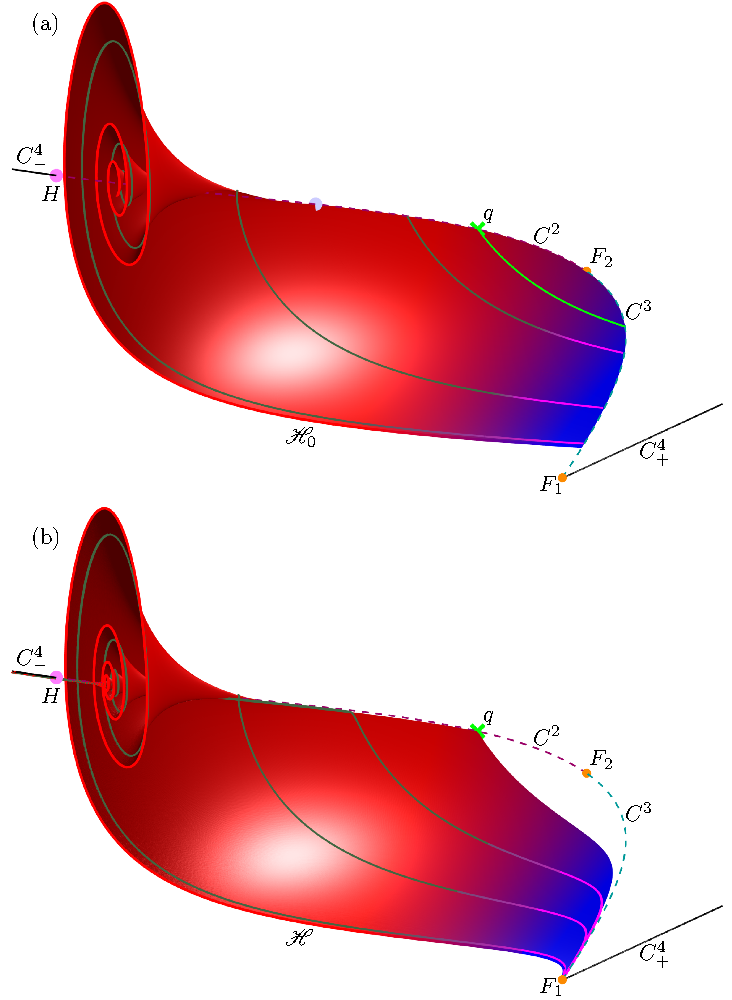
\includegraphics[]{./figures/MKMO_13.pdf}
\caption{Projections onto ($B$, $A$, $X$)-space of the portion of $\mathscr{H}_0$ lying in the region $B < 0.781$ (red-blue fade surface) (a) and of $\mathscr{H}$ for $\varepsilon=0.0037$ (red-blue fade surface) (b).   Also shown in panel (a) for $\varepsilon=0$ are the intersection $W^u(q)\cap\mathscr{H}_0$ (green curve) for $\varepsilon=0$ and the point $p \in C^2$ (periwinkle dot) with $p_B \approx 0.477$ where the eigenvalues become complex conjugate.   Both panels also show representative orbit segments (forest green-magenta fade curves), the equilibrium $q$ (green cross), the curves $C^2$, $C^3$, and $C^4_\pm$, and the points $F_1$, $F_2$, and $H$.}
\label{figure_13}
\end{figure}

Figure \ref{figure_13} shows in projection onto ($B$,$A$,$X$)-space the two computed surfaces $\mathscr{H}_0$ for $\varepsilon=0$ (red-blue fade surface) in panel (a) in comparison with the surface $\mathscr{H}$ for $\varepsilon=0.0037$ (red-blue fade surface) in panel (b).  To aid a visual comparison with $\mathscr{H}$ in panel (b), we show only the portion of $\mathscr{H}_0$ in panel (a) that lies in the region $B < 0.781$.  Notice how $\mathscr{H}_0$ starts to spiral increasingly from the equilibrium (periwinkle dot) on $C^2$ where the eigenvalues become complex conjugate.  Due to the $B$-dependence of $r_2$, the surface does not spiral all the way into $C^3$.  In both panels, three representative orbit segments are shown on the surface (forest green-magenta fade curves).  Unlike orbit segments on $\mathscr{H}$, orbit segments on $\mathscr{H}_0$ do not exhibit any drift in the direction along $C^2$ and $C^3$, respectively because $\varepsilon=0$ so that $B$ is constant.  The intersection of $\mathscr{H}_0$ with $W^u(q)$ (green curve) for $\varepsilon=0$ is analogous to the boundary of $\mathscr{H}$ near $q$; compare with Figure \ref{figure_12}.  The picture indicates that $\mathscr{H}_0$ and $\mathscr{H}$ are very close.  We checked this observation using integral norms in sections with fixed $B$-values; see the appendix for details.

%%MMO section
\section{Mixed-mode oscillations and their geometry}

We turn to the question of what role the surface of hetroclinic connections $\mathscr{H}$ plays for MMOs, which are characterized by having epochs of local small-amplitude oscillations (SAOs) followed by epochs of global large-amplitude oscillations (LAOs).  We begin by considering the periodic orbit $\Gamma$ for $\varepsilon=0.0037$, a value of $\varepsilon$ for which $\Gamma$ is an attracting MMO.  

\begin{figure}[H]
\centering
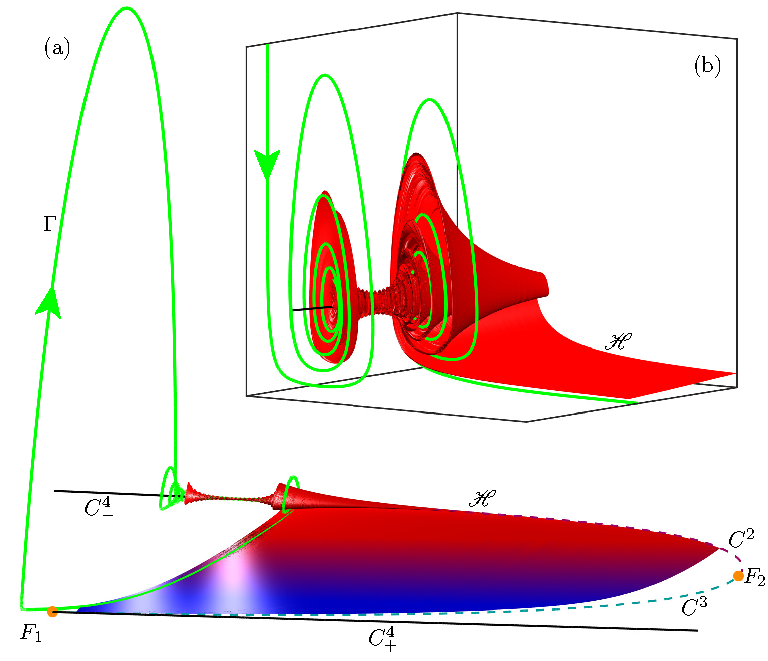
\includegraphics[]{./figures/MKMO_14.pdf}
\caption{The attracting MMO $\Gamma$ (green curve) and the surface of heteroclinic connections $\mathscr{H}$ (red-blue fade surface) for $\varepsilon=0.0037$ shown in projection onto ($B$,$A$,$X$)-space. The surface $\mathscr{H}$ is extended in backward time past the Hopf bifurcation point $H$.  Panel (a) shows the global view of $\Gamma$ tracking $\mathscr{H}$ from $C^2$ (dashed raspberry curve) to $C^3$ (dashed teal curve) and then transitioning back to $C^4_-$ (solid black curve) which constitutes the LAO.  Panel (b) shows an enlargement of the region where $\Gamma$ makes a subsequent slow passage through $H$ to generate SAOs.}
\label{figure_14}
\end{figure}

Figure \ref{figure_14} shows the attracting MMO $\Gamma$ (green curve) for $\varepsilon=0.0037$ in projection onto ($B$, $A$, $X$)-space with the surface $\mathscr{H}$ (red-blue fade surface) of heteroclinic connections, which has been extended in backward time past $H$.  Here the attractor $\Gamma$ was obtained by forward-time integration.  Figure \ref{figure_14}(a) shows a global view of $\Gamma$ and $\mathscr{H}$.  We observe $\Gamma$ entering into the region of SAOs near the attracting branch $C^4_-$ of $C$.  The MMO spirals as it enters the scroll-like region of $\mathscr{H}$, with increasingly smaller SAOs as it makes a slow passage through $H$ to $C^2$; note that $S^2$ is not distinguishable from $C^2$ at this scale.  On the other side of $H$, near $C^2$, we observe the SAOs increasing in size until $\Gamma$ leaves the region of SAOs.  An enlargement of the slow passage through $H$ is shown in panel (b).  In this enlargement, we also see $\Gamma$ exit the region of SAOs by spiralling out of the scrolls of $\mathscr{H}$ to the underside of the flatter part of $\mathscr{H}$ in between $C^2$ and $C^3$.  The global view in panel (a), shows that $\Gamma$ subsequently tracks an orbit segment on $\mathscr{H}$ at an intermediate speed to cross over to $C^3$; again, $S^3$ is not distinguishable from $C^3$ at this scale.  We find that $\Gamma$ extends slightly past the fold point $F_1$ before making a single LAO, mostly in the $X$- and $Y$-directions, back to the attracting slow manifold near $C^4_-$.  For this value of $\varepsilon$, the return mechanism of $\Gamma$ from a region of SAOs into a region of LAOs clearly involves $\mathscr{H}$.

\begin{figure}[H]
\centering
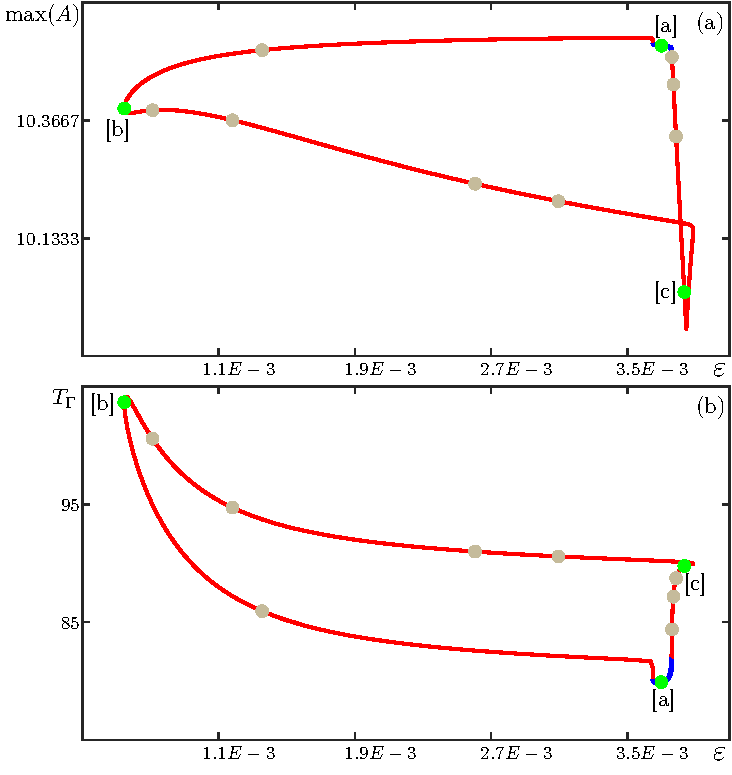
\includegraphics[]{./figures/MKMO_15.pdf}
\caption{Isola of periodic MMOs $\Gamma$ when $\varepsilon$ is varied, shown in terms of the maximum value of $A$ (a) and its period $T_\Gamma$ (b), respectively.  Here, $\Gamma$ is stable along the blue part and unstable along the red part of the isola.  Green dots labeled [a], [b], and [c] correspond to $\Gamma$ as shown in Figure \ref{figure_16}; these and the taupe dots correspond to MMOs shown in Figures \ref{figure_17} and \ref{figure_18}.}
\label{figure_15}
\end{figure}

Singular objects generally play a role in organizing the geometry of an MMO provided $\varepsilon$ is small enough; see \cite{MMO} for an overview and original references.  For this reason, we investigate the MMO periodic orbit $\Gamma$ for varying $\varepsilon$ and identify singular objects for $\epsilon=0$ that play a role in the MMO structure of $\Gamma$.  In particular, we always compare with the singular $\mathscr{H}_0$ for all $\varepsilon$-values from now on.  Singular limits of periodic MMOs can be investigated in many situations by continuing the corresponding periodic MMO for decreasing $\varepsilon$, ideally to $\varepsilon=0$ to connect with theoretical results \cite{Nonlinearity, MMO, Autocatalator}.  On the other hand, it is known from previous literature that MMO periodic orbits may also form isolas when other parameters are varied \cite{Nonlinearity, Forest_pest_model}.    Specifically for the Olsen model, isolas were found in \cite{QSSA} where a single parameter in their formulation was changed; in our context this would mean changing $\alpha$, $\varepsilon$, $\kappa$, and $\lambda$ simultaneously in a certain way; see \cite{Rescaling} for the exact parameter rescalings.

We find here that the MMO periodic orbit $\Gamma$ forms an isola when continued in $\varepsilon$; in particular, it does not reach $\varepsilon=0$ but rather extends only to the minimum of $\varepsilon \approx 0.00055$.  Moreover, the periodic orbit $\Gamma$ exists only for a narrow range of $\varepsilon$ with a maximum of $\varepsilon \approx 0.00389$.  Nevertheless, the properties of $\Gamma$ change as $\varepsilon$ progresses around the isola.  Figure \ref{figure_15} shows the isola (red and blue curve) of $\Gamma$ over $\varepsilon$, with the vertical axis representing the maximum value along $\Gamma$ of the $A$-coordinate in panel (a) and the period of $\Gamma$, denoted $T_\Gamma$, in panel (b).  The blue segment of the isola indicates where $\Gamma$ is stable and along the red segment $\Gamma$ has at least one unstable Floquet multiplier and is, hence, unstable.  The green dot labeled [a] corresponds to the original stable MMO shown in Figure \ref{figure_14}, the green dot labeled [b] lies on the isola's minimum in $\varepsilon$ which is also a fold point, and the green dot labeled [c] is chosen such that the corresponding MMO is representative of a particularly interesting geometry of $\Gamma$ that will be discussed in the following paragraphs.  The MMO periodic orbits at the green dots labeled [a]-[c] are shown in Figure \ref{figure_16} together with $\mathscr{H}_0$ and other singular objects introduced below.  Moreover, Figure \ref{figure_17} shows projections onto the ($B$, $A$)-plane of $\Gamma$ and the singular objects at the green dots [a]-[c], as well as at the intermediate taupe dots of Figure \ref{figure_15}; Figure \ref{figure_18} shows the corresponding time traces of the $X$-coordinates of the MMOs.

\begin{figure}[H]
\centering
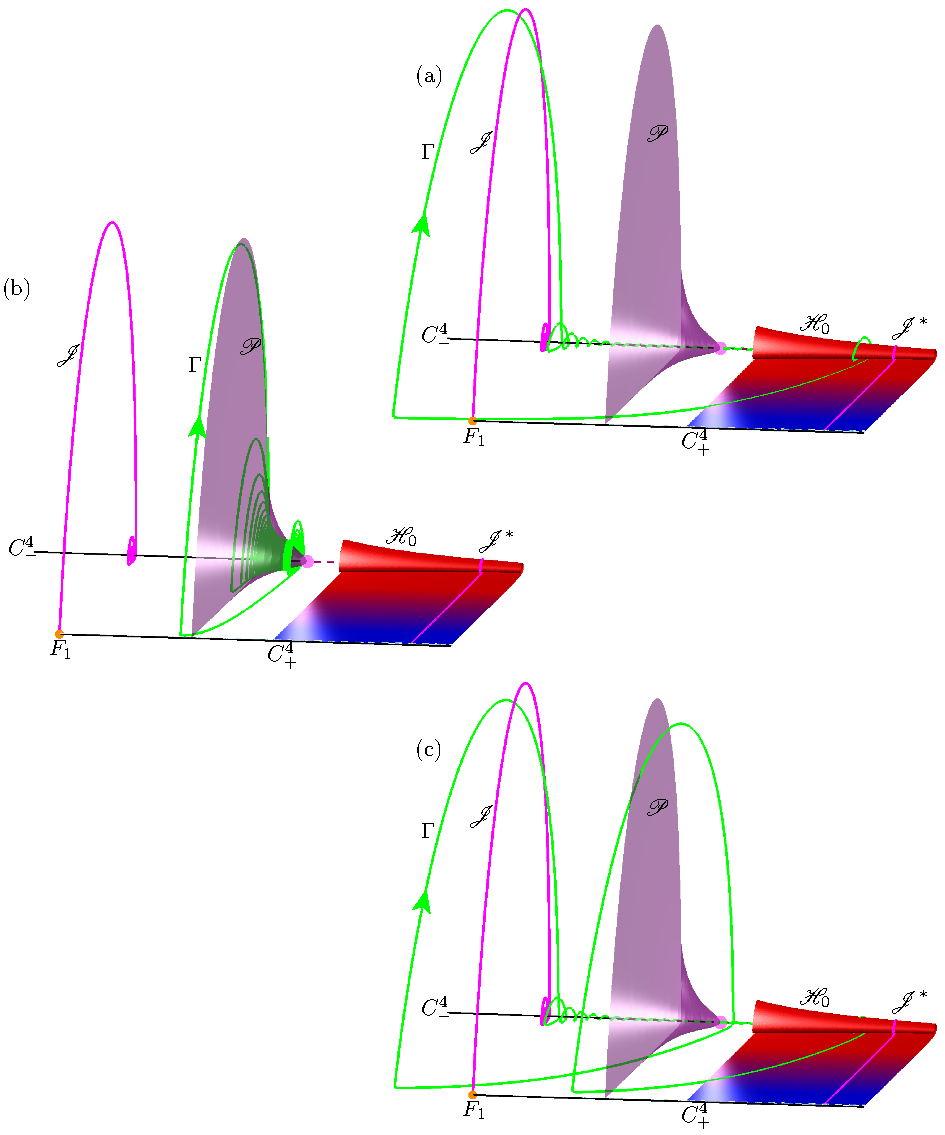
\includegraphics[]{./figures/MKMO_16.pdf}
\caption{The periodic MMO $\Gamma$ (green curve) shown in projection onto ($B$, $A$, $X$)-space with the portion of $\mathscr{H}_0$ (red-blue fade surface) lying in the region $B<0.781$, the jump-back trajectory $\mathscr{J}$ (magenta curve) and its dual $\mathscr{J}^*$ (magenta curve), and the surface $\mathscr{P}$ of singular periodic orbits (midnight-grape surface).  Also shown are $C^2$, $C^3$, $C^4_\pm$, $F_1$, $F_2$, and $H$.  Panel (a) shows $\Gamma$ for the orignal value of $\varepsilon=0.0037$ and panels (b) and (c) show $\Gamma$ for $\varepsilon=0.00055$ and $\varepsilon=0.00383$ at the points labeled [b] and [c] in Figure 15, respectively.}
\label{figure_16}
\end{figure}

Figure \ref{figure_16} shows $\Gamma$ in projection onto ($B$,$A$,$X$)-space for three values of $\varepsilon$ in relation to several limiting objects.  Specifically, we show portions of $C^2$, $C^3$, $C^4_\pm$, $\mathscr{H}_0$, and three additional singular objects.  The singular jump orbit $\mathscr{J}$ (magenta curve) is the solution of the reduced system (\ref{equation_2}) that connects the point $F_1$ to the branch $C^4_-$; indeed, the corresponding point on $C^4_-$ is the only attractor for this value of $B$.  The dual of $\mathscr{J}$, denoted $\mathscr{J}^*$ (magenta curve), is a trajectory on $\mathscr{H}_0$ that lies at an equal distance away from $H$ in the $B$-direction.  We refer to $\mathscr{J}^*$ as the dual of $\mathscr{J}$ because, in the limit of $\varepsilon$ equal to $0$, the drift in $B$ along $C^4_-$ from $\mathscr{J}$ to $H$ takes the same time as the drift in $B$ along $C^2$ from $H$ to $\mathscr{J}^*$.  A surface $\mathscr{P}$ of singular saddle periodic orbits (midnight-grape surface) originates from $H$ and ends at a homoclinic connection to an equilibrium on $C^3$.  Each periodic orbit for fixed $B$ on the surface $\mathscr{P}$ has a two-dimensional stable and a two-dimensional unstable manifold.  Hence, the surface $\mathscr{P}$ has a three-dimensional stable and unstable manifolds.

Figure \ref{figure_16}(a) shows the attracting MMO $\Gamma$ for the original value of $\varepsilon=0.0037$, the same as in Figure \ref{figure_14} and corresponding to the green dot labeled [a] in Figure \ref{figure_15}.  As in Figure \ref{figure_14}, $\Gamma$ is seen to enter into the region of SAOs near the attracting branch $C^4_-$ of $C$ exhibiting decreasing SAOs as it spirals through the surface $\mathscr{P}$ of singular periodic orbits. The SAOs increase as $\Gamma$ passes $\mathscr{P}$ near the Hopf point $H$.  Then $\Gamma$ exits the region of SAOs by following $\mathscr{H}_0$ closely to a region near $C^3$ (illustrating again the closeness of $\mathscr{H}_0$ and $\mathscr{H}$ at this scale).  It extends past $F_1$ before making an LAO back to $C^4_-$.  The single LAO somewhat tracks the singular jump orbit $\mathscr{J}$ (magenta curve) from $F_1$ to $C^4_-$.  We also observe that $\Gamma$ exits the region of SAOs near its dual $\mathscr{J}^*$ (magenta curve).  These observations are consistent with our expectation that the SAOs are due to the tourbillon mechanism of passage through a Hopf bifurcation as described in \cite{MMO} and, in particular, the distance between $H$ and where $\Gamma$ enters the region of SAOs is similar to the distance between $H$ and where $\Gamma$ leaves it.  This also means that the number of SAOs exhibited by $\Gamma$ before reaching $H$ is approximately the same as the number of SAOs exhibited after passing it.  Overall, Figure \ref{figure_16}(a) suggests that $\mathscr{J}$, $\mathscr{J}^*$, and appropriate portions of $C^2$, $C^3$, $C^4_\pm$, and $\mathscr{H}_0$ may act as a singular limit for $\Gamma$.

Figure \ref{figure_16}(b) shows $\Gamma$ for the smaller value of $\varepsilon=0.00055$, corresponding to the green dot labeled [b] in Figure \ref{figure_15}.  We see $\Gamma$ entering the region of SAOs via the attracting branch $C^4_-$.  The periodic orbit $\Gamma$ now closely follows the surface of singular periodic orbits $\mathscr{P}$ generating large SAOs in the process.  Notice that $\Gamma$ does not pass near $H$, but passes through $\mathscr{P}$ in the ($B$, $A$, $X$)-projection.  The MMO then follows the two-dimensional intersection of $W^s(C^3)$ and the unstable manifold of $\mathscr{P}$ (not shown) away from $\mathscr{P}$ toward $C^3$.  As the MMO crosses the region between $C^4_-$ and $C^3$, it exhibits minimal drift in the $B$-direction due to the smaller value of $\varepsilon$, compare with panel (a).  Almost immediately after reaching $C^3$, $\Gamma$ makes an LAO that tracks the singular homoclinic connection which limits the surface $\mathscr{P}$, back to the region of SAOs.  The MMO shown in panel (b) features a much narrower range of $B$-values than the one shown in panel (a) while the amplitude of the SAOs is larger.  Our observations of panel (b) suggest that $\Gamma$ has $\mathscr{P}$ as a singular limit, which corresponds to a much more localized phenomenon.

Figure \ref{figure_16}(c) shows $\Gamma$ for the larger value of $\varepsilon=0.00383$, corresponding to the green dot labeled [c] in Figure \ref{figure_15}.  As in Figure \ref{figure_16}(a), $\Gamma$ enters the region of SAOs near where $\mathscr{J}$ meets $C^4_-$, transitions through $H$ to $C^2$, exits the region of SAOs near $\mathscr{J}^*$, and follows $\mathscr{H}_0$ to $C^3$.  Upon reaching $C^3$ well before $F_1$, the MMO $\Gamma$ has an LAO that quickly takes it back to $C^2$ rather than to $C^4_-$.  Without exhibiting any SAOs, it then drifts back to $C^3$ and has a second LAO starting well past $F_1$, very much like the LAO of the MMO in panel (a).  For this MMO it is unclear what role the singular limits play in the organization of the MMO.

\begin{figure}[H]
\centering
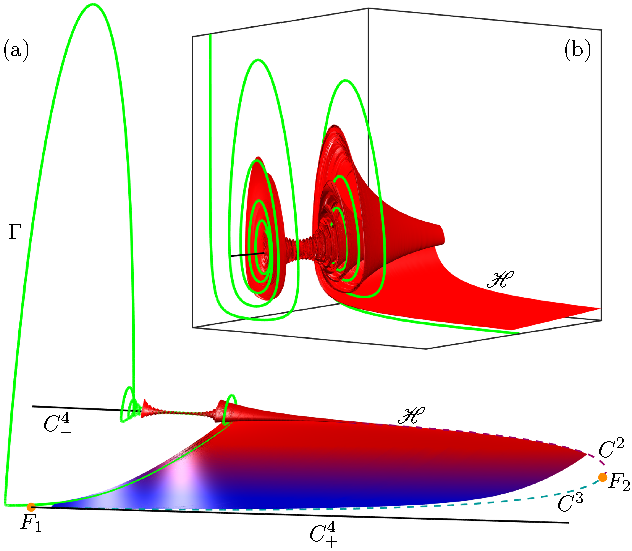
\includegraphics[]{./figures/MKMO_17.pdf}
\caption{Projections onto the ($B$, $A$)-plane of the MMO $\Gamma$ (green curve) showing its evolution when varying $\varepsilon$ counter-clockwise around the isola in Figure \ref{figure_15}.  Panels with labels [a], [b], and [c], and those without labels correspond to the labelled and taupe dots in Figure \ref{figure_15}, respectively; compare also with Figure \ref{figure_16}.  Also shown are $\mathscr{J}$ and $\mathscr{J}^*$ , $\mathscr{P}$, $F_1$, $H$, and segments of $C^2$, $C^3$, and $C^4_\pm$; see their labels in the first panel.}
\label{figure_17}
\end{figure}

Figure \ref{figure_16} illustrates that the behavior of $\Gamma$ changes significantly around the isola.  A natural question is then how $\Gamma$ deforms continuously as we move around the isola shown in Figure \ref{figure_15}.  The change in geometry is shown in finer detail in the panels of Figure \ref{figure_17}, which can be imagined as stills of an animation as the isola is traversed in a counter-clockwise direction.  Each panel shows $\Gamma$ for successive values along the isola, beginning and ending at the original value $\varepsilon=0.0037$.  Here we show the projection onto the ($A$,$X$)-plane, also the singular objects $\mathscr{J}$, $\mathscr{J}^*$, $\mathscr{P}$, $F_1$, $H$, and relevant portions of $C$.  The MMO periodic orbits shown in panels labeled [a], [b], and [c] correspond to the instances of $\Gamma$ shown in Figures \ref{figure_16}(a), (b), and (c); values of $\varepsilon$ shown in Figure \ref{figure_17} are labelled or taupe dots in Figure \ref{figure_15}.  The first and last panels are identical and labeled [a] to illustrate the beginning and return to $\Gamma$ at the original $\varepsilon=0.0037$.  To illustrate the associated MMOs, Figure \ref{figure_18} shows the time evolution of the $X$-coordinate over one period of $\Gamma$ along the isola for the exact same values of $\varepsilon$, again imagined as stills of an animation.  Here, the horizontal axis is the rescaled time variable $t \in [0,1]$ and the period $T_\Gamma$ of the periodic MMO is shown above the time series in each panel of Figure \ref{figure_18}.

The first row of panels in Figures \ref{figure_17} and \ref{figure_18} illustrates the transition of $\Gamma$ from $\varepsilon=0.0037$ at [a] to $\varepsilon=0.00055$ at [b].  Note in Figure \ref{figure_17} how the $B$-direction narrows continuously and the amplitude of SAOs increases.  In the process, $\Gamma$ makes an earlier fast exit from the region of $C^3$, well before reaching the point $F_1$.  The intermediate panel is a good example of a tourbillon mechanism with a nearly symmetrical change in sufficiently large amplitude of the SAOs on either side of $H$.  As a result, the periodic MMO $\Gamma$ for $\varepsilon=0.00055$ at [b] is quite localized near the point $H$; compare with Figure \ref{figure_16}(b) and note that $\Gamma$ lies entirely to one side of $H$.  The corresponding panels in Figure \ref{figure_18} clearly illustrate the increasing amplitude of SAOs; notice also the reducing frequency of SAOS as $\varepsilon$ decreases.

The subsequent transition from [b] to [c] is shown in the second and third rows, up to the middle panel in the third row of Figures \ref{figure_17} and \ref{figure_18}.  The main feature is that the outermost SAO increases in amplitude to become a second LAO.  Already for $\varepsilon=0.00071$, the largest SAO immediately after the LAO has increased so much in amplitude that we refer to it as an LAO.  This is seen even more clearly in Figure \ref{figure_18}, where there is a gap in the time series between LAOs.  As $\varepsilon$ is increased further, to $\varepsilon=0.00118$, it is clear that this panel looks like the panel directly above it with an additional LAO on the left.  The first LAO back to $C^4_-$ is initially to the right of $H$ in Figure \ref{figure_17}, but it moves left as $\varepsilon$ is increased and the first LAO occurs earlier and earlier until it is approximately at $H$ in panel [c].  Corresponding panels in Figure \ref{figure_18} show the distance between LAOs increasing and the tourbillon mechanism decreasing in amplitude.

The remaining panels of Figures \ref{figure_17} and \ref{figure_18} show the transition from [c] back to [a].  The tourbillon mechanism does not change in these panels, the only change we observe is an increasing gap between the first and second LAO until the distance between the last SAO and the first LAO is much smaller than the distance between LAOs.  In this process, the amplitude of the first LAO decreases substantially until it is of the same magnitude of the last SAO and we refer to it as an SAO.  This increase in the distance between LAOs corresponds, in Figure \ref{figure_17}, to the the first return to $C^4_-$ after the SAOs moving well to the left of $H$.  We can see the decrease of the maximum $A$-value in Figure \ref{figure_17} for the first, left-most LAO until we return to the periodic MMO $\Gamma$ back at [a].  A similar decrease of the $X$-coordinate can be observed on the corresponding panels of Figure \ref{figure_18}.

\begin{figure}[H]
\centering
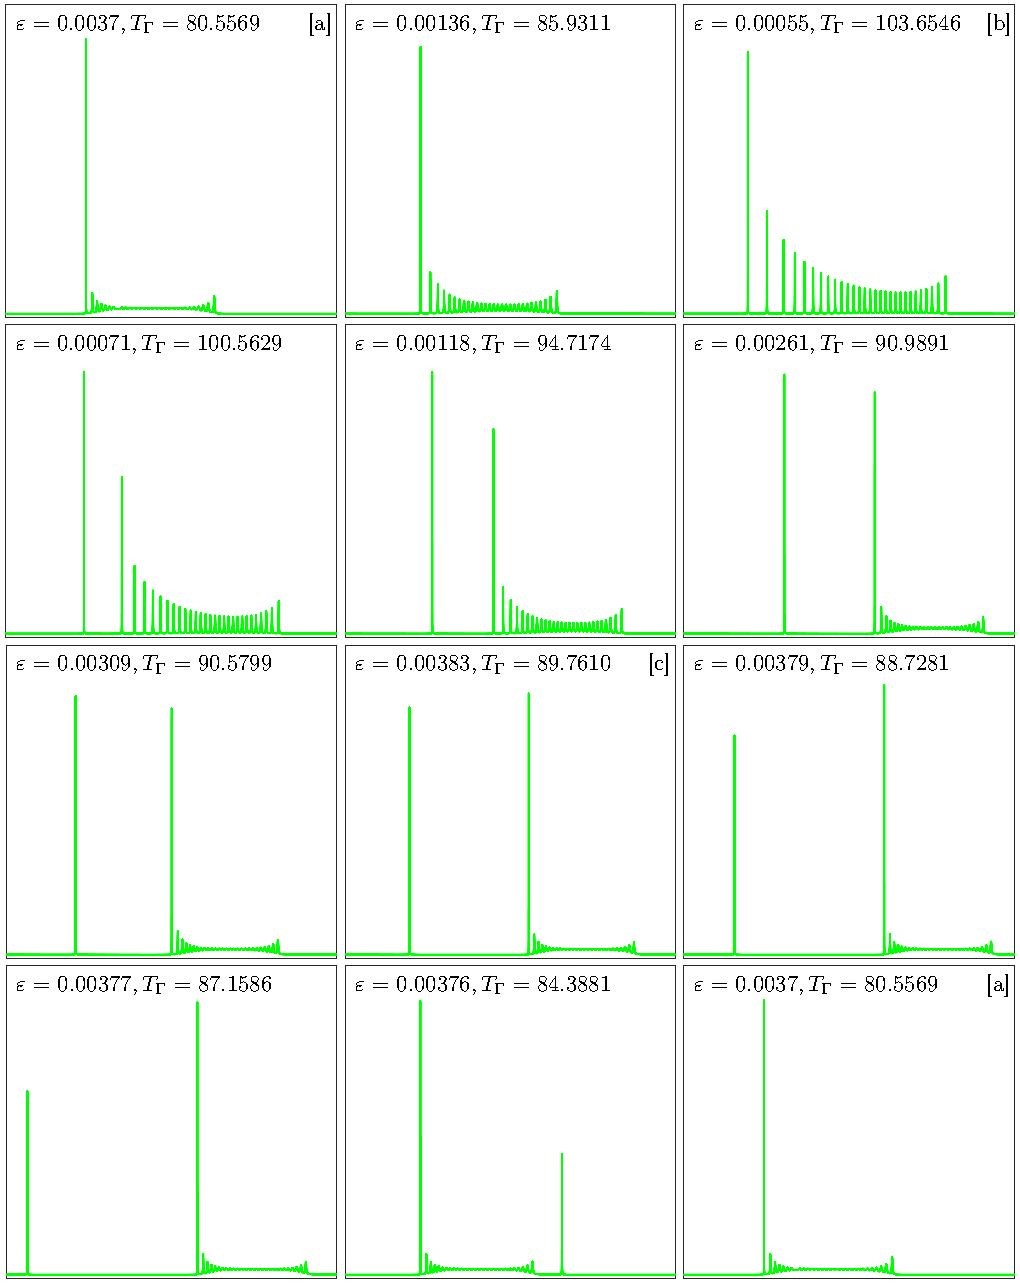
\includegraphics[]{./figures/MKMO_18.pdf}
\caption{Time series of the $X$-coordinate of the periodic MMO $\Gamma$ over one period $T_\Gamma$ (shown at top of panels) for varying $\varepsilon$; the individual panels correspond directly to those of Figure \ref{figure_17}.}
\label{figure_18}
\end{figure}

In summary, we find that the periodic MMO $\Gamma$ changes considerably along the $\varepsilon$-isola in the following way: SAOs grow and then shrink in amplitude, generating a second LAO in the process that splits on one side and then rejoins on the other.  Moreover, we see that the singular limits that influence the geometry of $\Gamma$ change as $\Gamma$ makes its way around the isola.  For $\varepsilon=0.00055$ and other relatively small values of $\varepsilon$, we find that the singular surface $\mathscr{P}$ has the most influence over the geometry of $\Gamma$.  For the original value $\varepsilon=0.0037$, as well as other relatively large values of $\varepsilon$, on the other hand, the singular objects $\mathscr{J}$, $\mathscr{J}^*$, and $\mathscr{H}_0$ play this role.  In particular, for larger values of $\varepsilon$, the surfaces $\mathscr{H}_0$ and $\mathscr{H}$ of heteroclinic connections are integral to the return of $\Gamma$ from a region of SAOs to a region of LAOs and back to SAOs.  We conclude that the surface of heteroclinic connections is part of a previously unknown mechanism for the generation of MMOs in a four-dimensional phase space.

\newpage

\section{Conclusions}

We investigated a mechanism for an attracting periodic mixed-mode oscillation (MMO) $\Gamma$ in the four-dimensional Olsen model for peroxidase-oxidase reaction in a parameter regime corresponding to one slow and three fast variables.  The geometry of $\Gamma$ was of particular interest because it was unlike what has previously been observed in lower-dimensional systems.

We first presented an algorithm for computing two-dimensional submanifolds of three-dimensional stable and unstable manifolds of saddle slow manifolds.  Our approach was based on computing one-parameter families of solutions to two-point boundary value problems (2PBVPs).  Submanifolds were selected with boundary conditions and were computed in a neighbourhood of two saddle slow manifolds of different type in the Olsen model.  The geometry of the submanifolds revealed an intermediate time-scale along which variables evolve.

We next presented how Lin's method can be implemented to compute the structurally stable surface $\mathscr{H}$ of heteroclinic connections resulting from the two-dimensional intersection of a three-dimensional stable manifold of a saddle slow manifold and three-dimensional unstable manifold of a different saddle slow manifold.  This was again based on a 2PBVP approach to computing a one-parameter family of solutions with appropriate boundary conditions.  Even though our choice of parameters for system (\ref{equation_1}) places it in the class of systems with three fast variables according to \cite{Rescaling}, we found that orbits on the surface of heteroclinic connections evolve on a third, intermediate time-scale.  We found that $\mathscr{H}$ transports $\Gamma$ at an intermediate speed from a region of small-amplitude oscillations (SAOs) near a Hopf bifurcation of the fast subsystem into a region of large-amplitude oscillations (LAOs) at the end of the other saddle slow manifold.  The surface $\mathscr{H}$ is thus an important ingredient in the mechanism for the generation of $\Gamma$ and is responsible for a portion of its novel geometry.  Whether $\mathscr{H}$ is responsible for the generation of a localized intermediate time-scale that isn't present globally for system (\ref{equation_1}) remains to be explored.

Using standard methods for computing heteroclinic connections between equilibria, we additionally computed the limiting surface to which $\mathscr{H}$ converges as the original time-scale parameter $\varepsilon$ approaches zero.  It was found that the integral norm between this surface, denoted $\mathscr{H}_0$, and $\mathscr{H}$ was sufficiently small for $\mathscr{H}_0$ to serve as a good approximation of $\mathscr{H}$ for small $\varepsilon$.  With this in mind, we continued $\Gamma$ in $\varepsilon$ and compared the periodic MMOs with $\mathscr{H}_0$.  We discovered, in continuing $\Gamma$, that $\Gamma$ lies on an isola in $\varepsilon$ and has a unique bifurcation structure.  As the isola in $\varepsilon$ is traversed, $\Gamma$ changes type by increasing SAOs in amplitude until they become LAOs and vice-versa.  It is unknown whether MMOs associated with heteroclinic surfaces generally bifurcate by means of increasing and decreasing oscillation amplitude or if varying time-scaling parameters might give rise to different bifurcation structures.

We then compared representative $\Gamma$ on the isola with $\mathscr{H}_0$ and several other singular objects.  Through these comparisons, it was observed that the singular limit of $\Gamma$ changes as $\varepsilon$ varies.  For the original value of $\varepsilon=0.0037$, we observe $\Gamma$ tracking $\mathscr{H}_0$. For a much smaller $\varepsilon$, it was found that $\Gamma$ primarily tracks a surface of singular periodic orbits.   At this time, the singular limits that influence intermediate $\Gamma$ between these two examples remain to be explored.

Our results inspire several questions for future direction.  The singular limits affecting the geometries of $\Gamma$ for intermediate values of $\varepsilon$ have yet to be investigated and other singular limits may contribute to the geometry as one changes multiple parameters simultaneously.  Changing multiple parameters may be the key to extending the isola on which $\Gamma$ lies to $\varepsilon=0$.  Changing $\varepsilon$ alone may not be sufficient to obtain a complete picture of the singular limits organizing $\Gamma$ as the finite time-scale difference between variables $X$, $Y$, and $A$ may cause the Olsen model to behave more as a three-time-scale system than previously assumed.  Increasing the speed of the time-scale on which $A$ evolves would be one way to make the Olsen model more of a true two-time-scale system; this the subject of ongoing work where we hope to also explore the prevalence of the bifurcation structure of $\Gamma$ and determine whether three time-scales are essential for the existence of $\mathscr{H}_0$ and a geometry such as $\Gamma$.

\newpage

\section{Appendix}

\subsection*{Defining the Distance of $\mathscr{H}$ from $\mathscr{H}_0$}

Fenichel theory implies that $\mathscr{H}$ converges to $\mathscr{H}_0$ with decreasing $\varepsilon$ \cite{Fenichel}.  A natural question is then how close $\mathscr{H}_0$ and $\mathscr{H}$ are to each other for $\varepsilon=0.0037$.  To investigate the distance of $\mathscr{H}$ from $\mathscr{H}_0$, we stratify the surfaces into intersections with sections $\Lambda = \{ \omega \in \mathbb{R}^4 \; | \; \omega_B = \widehat{B}\}$ for several values of $\widehat{B}$.  We denote intersections $\mathscr{H} \cap \Lambda := \mathscr{H}^{\widehat{B}}$ and $\mathscr{H}_0 \cap \Lambda := \mathscr{H}_0^{\widehat{B}}$, respectively.  The $\widehat{B}$-dependent integral norm of the difference between $\mathscr{H}^{\widehat{B}}$ and $\mathscr{H}_0^{\widehat{B}}$  in $\Lambda$ can then be computed to give an idea of the distance of $\mathscr{H}$ from $\mathscr{H}_0$.

Any $\mathscr{H}_0^{\widehat{B}}$ can be readily obtained by including the requirement that $B=\widehat{B}$ in the computation of $\mathscr{H}_0$.  We increase the mesh size for accuracy in the computation and take $r_2=1\times10^{-3}$.  Since we do not intend to render a surface after the computation of $\mathscr{H}_0^{\widehat{B}}$, it is not necessary to keep the mesh size constant for all $\widehat{B}$.

To compute $\mathscr{H}^{\widehat{B}}$, we could use a computer package such as $\textsc{MATLAB}$ to approximate the intersection curve $\mathscr{H}^{\widehat{B}} = \mathscr{H} \cap \Lambda$ from the data of the computed surface $\mathscr{H}$.  However it is much more accurate and elegant to compute $\mathscr{H}^{\widehat{B}}$ via continuation.  The computation of $\mathscr{H}^{\widehat{B}}$ works as follows.  We first follow the steps for computing $\mathscr{H}$ and stop the continuation when $\mathbf{u}(0)_B = \widehat{B}$ instead of sweeping out the entire surface.  We then replace conditions (\ref{general_conditions_heteroclinic_1}) and (\ref{general_conditions_heteroclinic_2}) with the new boundary conditions
	\begin{equation}
		\mathbf{u}(0) \in \Lambda
		\label{general_conditions_intersection_1}
	\end{equation}
and
	\begin{equation}
		\mathbf{w}(0) \in \Lambda
		\label{general_conditions_intersection_2}
	\end{equation}	
and continue the one-parameter family of paired orbit segments ($\mathbf{w}$, $\mathbf{u}$) satisfying (\ref{general_conditions_heteroclinic_3}), (\ref{general_conditions_heteroclinic_4}), (\ref{general_conditions_heteroclinic_5}), (\ref{general_conditions_heteroclinic_6}), (\ref{general_conditions_intersection_1}), and (\ref{general_conditions_intersection_2}) with varying $\mathbf{u}(0)_A$ and $T$.  The curve $\mathscr{H}^{\widehat{B}}$ is then given as the one-parameter family $\mathbf{u}(0)$.

\begin{figure}[H]
\centering
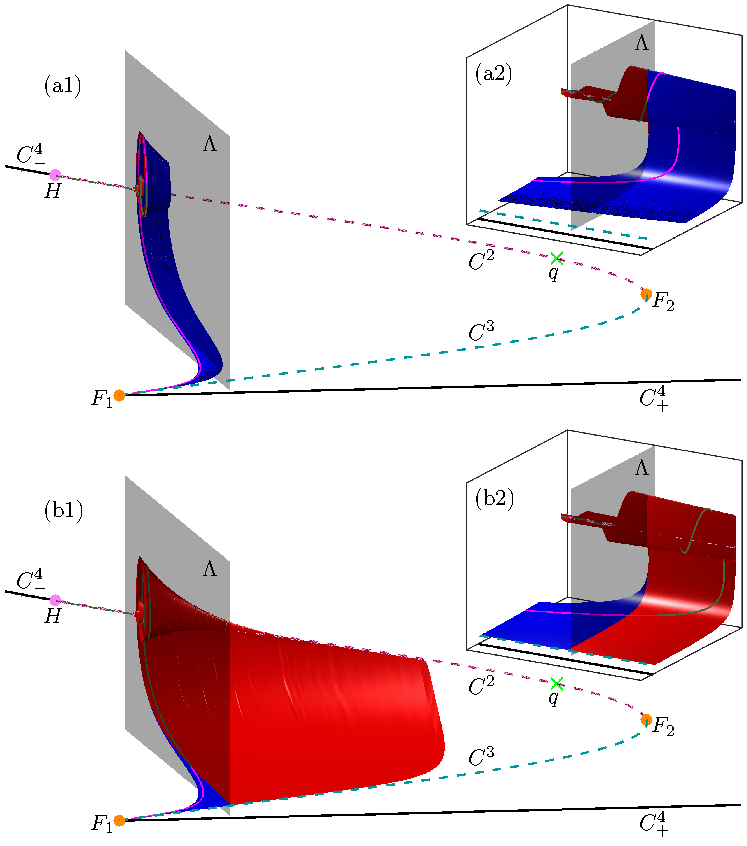
\includegraphics[]{./figures/MKMO_19.pdf}
\caption{Computation of the intersection $\mathscr{H}^{\widehat{B}}$ in $\Lambda$ (charcoal surface) for $\widehat{B}=0.75$, shown in projection onto $(B, A, X)$-space.  Shown are one-parameter families of paired orbit segments ($\mathbf{u}$, $\mathbf{w}$), with $\mathbf{w}$ colored red as a surface and forest-green as a curve, and $\mathbf{u}$ colored blue as a surface and magenta as a curve.  Panels (a1) and (a2) show paired orbit segments ($\mathbf{w}$,$\mathbf{u}$) (forest green/magenta curves) for which $\mathbf{u}(0) \in \Lambda$ on the right-hand side.  Panels (b1) and (b2) shows paired orbit segments ($\mathbf{w}$,$\mathbf{u}$) where $\mathbf{u}(0) \in \Lambda$ on the left-hand side.  The pieces were computed as a one-parameter family of ($\mathbf{w}$, $\mathbf{u}$) with $\mathbf{u}(0)$ capturing the first intersection of ($\mathbf{w}$, $\mathbf{u}$) with $\Lambda$ (charcoal surface) (a) and with $\mathbf{u}(0)$ capturing the second intersection of ($\mathbf{w}$, $\mathbf{u}$) with $\Lambda$ (b).  Global views of the pieces of $\mathscr{H}$ are shown in panels (a1) and (b1).  Enlargements of the region near $\mathscr{H} \cap \Lambda$ are shown in panels (a2) and (b2).}
\label{figure_19}
\end{figure}

The three-dimensional section $\Lambda$ is divided into two regions by a two-dimensional surface of points at which the vector field (\ref{equation_1}) is tangent to $\Lambda$ in the $B$-direction.  This surface, called a tangency locus \cite{tangency_locus_paper}, slices the curve $\mathscr{H}^{\widehat{B}}$ into two parts: one on which the vector field (\ref{equation_1}) flows from left to right (from larger to smaller values of $B$) through $\mathscr{H}^{\widehat{B}}$ and the other on which the vector field flows from right to left.  Our algorithm computes both pieces of $\mathscr{H}^{\widehat{B}}$, corresponding to the pieces of $\mathscr{H}$, shown in Figure \ref{figure_19}, in a single run.  The two pieces of $\mathscr{H}^{\widehat{B}}$ correspond to two pieces of $\mathscr{H}$ which are distinguished by the properties of the paired orbit segments ($\mathbf{w}$, $\mathbf{u}$).  Each panel of Figure \ref{figure_19} shows one of the two pieces of $\mathscr{H}$ computed for $\widehat{B}=0.75$ with the $\mathbf{w}$-family plotted in red and the $\mathbf{u}$-family plotted in blue.  Panel (a1) shows a global view of the portion of $\mathscr{H}$ for which the flow moves from left to right through $\mathbf{u}(0) \in \mathscr{H}^{\widehat{B}}$.  Panel (a2) shows an enlargement of the region where $\mathscr{H}$ intersects $\Lambda$.  An example orbit segment is shown in forest green and magenta and we can see that $\mathbf{u}(0)$ lies in the spiralling region of $\mathscr{H}$. Panel (b1) shows a global view of the portion of $\mathscr{H}$ for which the flow through $\mathbf{u}(0)$ moves from right to left.  Panel (b2) shows an enlargement of the region where $\mathscr{H}$ intersects $\Lambda$, and we can see from an example orbit segment that $\mathbf{u}(0)$ lies in a non-spiralling region of $\mathscr{H}$.  The orbit segments $\mathbf{u}$ that are to the right of $\Lambda$ in panels (a1) and (a2) correspond to the orbit segments $\mathbf{w}$ to the right of $\Lambda$ in panels (b1) and (b2).  The pieces of $\mathscr{H}$ shown in Figure \ref{figure_19}(a1) and Figure \ref{figure_19}(b1) do not constitute the entire surface $\mathscr{H}$.  This is due to the strong contraction in backward time near $C^2$ that causes many ($\mathbf{w}$, $\mathbf{u}$) pairs to be numerically indistinguishable with respect to the value for $\mathbf{u}(0)$.

\begin{figure}[H]
\centering
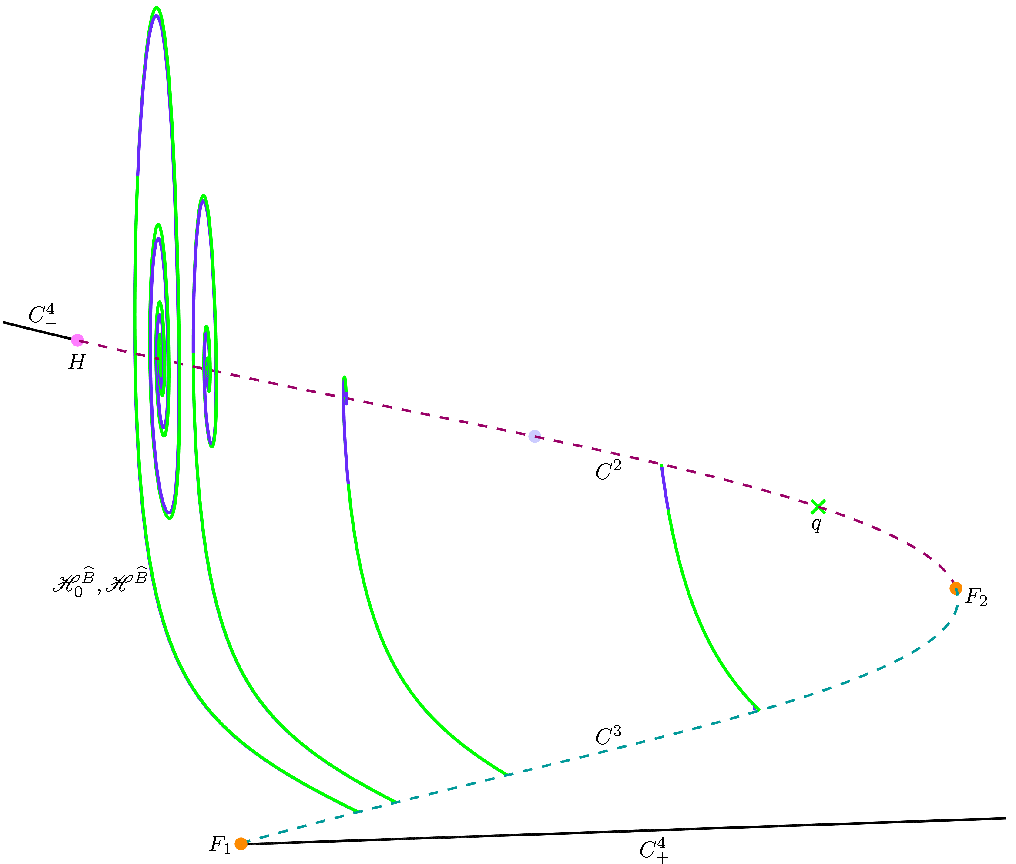
\includegraphics[]{./figures/MKMO_20.pdf}
\caption{Projection into ($B$, $A$, $X$)-space of the intersection curves $\mathscr{H}^{\widehat{B}}$ (royal purple) of $\mathscr{H}$ and $\mathscr{H}_0^{\widehat{B}}$ (green) of $\mathscr{H}_0$ with $\Lambda$ for $\widehat{B}=0.8$, $\widehat{B}=0.75$, $\widehat{B}=0.62$, and $\widehat{B}=0.4$ (left to right).  The curve $\mathscr{H}^{\widehat{B}}$ is visible behind $\mathscr{H}^{\widehat{B}}_0$ only in the region where the curves are spiralling.}
\label{figure_20}
\end{figure}

With the computational approach outlined above, we compare $\mathscr{H}_0^{\widehat{B}}$ and $\mathscr{H}^{\widehat{B}}$ inside $\Lambda$ for several choices of $\widehat{B} \in (H_B, F_{1_B})$.  Figure \ref{figure_20} shows intersection curves $\mathscr{H}_0^{\widehat{B}}$ (green) plotted on top of $\mathscr{H}^{\widehat{B}}$ (purple) for $\widehat{B}=0.8$, $\widehat{B}=0.75$, $\widehat{B}=0.62$, and $\widehat{B}=0.4$ (left to right) in projection into ($B$, $A$, $X$)-space.  Recall that the boundary of $\mathscr{H}^{\widehat{B}}_0$ is $(C^2 \cup C^3) \cap \Lambda$ and the boundary of $\mathscr{H}^{\widehat{B}}$ is $(S^2 \cup S^3) \cap \Lambda$.  Therefore, differences in the boundary points of  $\mathscr{H}^{\widehat{B}}$ and $\mathscr{H}_0^{\widehat{B}}$ are expected, because $S^3$ and $S^2$ lie $O(\varepsilon)$ away from $C^3$ and $C^2$, respectively.  The difference between boundary points of $\mathscr{H}^{\widehat{B}}$ and boundary points of $\mathscr{H}_0^{\widehat{B}}$ is only visible in the case of $\widehat{B}=0.4$.  Near $S^3$, the boundary point of $\mathscr{H}_0^{\widehat{B}}$ has a larger $A$-value, and, in the spiralling region near $S^2$, the boundary point of $\mathscr{H}_0^{\widehat{B}}$ has a smaller $A$-value than the boundary points of $\mathscr{H}^{\widehat{B}}$.    There is a noticeable difference in the curves farther away from the boundary points in areas where $\mathscr{H}^{\widehat{B}}_0$ and $\mathscr{H}^{\widehat{B}}$ spiral.  We can see that more spirals correspond to a larger distance between the curves.  The difference in $\mathscr{H}^{\widehat{B}}$ and $\mathscr{H}_0^{\widehat{B}}$ is more pronounced for $\widehat{B}$ closer to $H_B$ because $\mathscr{H}^{\widehat{B}}$ and $\mathscr{H}_0^{\widehat{B}}$ spiral more as $\widehat{B}$ approaches $H_B$.

We approximate the integral norm between $\mathscr{H}^{\widehat{B}}$ and $\mathscr{H}_0^{\widehat{B}}$ as a sum after mesh discretization.  To this end, we assign a mesh of size $N$ to $\mathscr{H}_0^{\widehat{B}}$ and index mesh points, denoted by $l_i$, from $1$ to $N$, starting from those closest to $C^3$.  This can be accomplished by fitting a spline $Spl_0$ to the computed data points on $\mathscr{H}_0^{\widehat{B}}$, obtained by continuation with $\textsc{Auto}$.  Desired mesh points can then be computed with $Spl_0$ at desired arclengths along $\mathscr{H}_0^{\widehat{B}}$.  For each $l_i \in \mathscr{H}_0^{\widehat{B}}$, we find an associated point $k_i \in \mathscr{H}^{\widehat{B}}$.  The norm is then the average distance between the point pairs.  This discretisation of the integral norm is the sum
	\begin{equation*}
		d\widehat{B} := \frac{1}{N} \sum_{i=1}^{N} \left \lVert l_i - k_i\right \lVert.
		\label{integral_norm}
	\end{equation*}
We also measure the distance between the two end points in the spiralling region for $\mathscr{H}_0^{\widehat{B}}$ and $\mathscr{H}^{\widehat{B}}$, which we denote by $\Delta_{\widehat{B}}$.

A fundamental difficulty in computing the integral norm is that for every $l_i$, we need to make a choice of how to find a unique $k_i$.  This is not straightforward because there is no general way of choosing a coordinate system that defines the distance of one curve to another.  The coordinate system we use is the one defined by perpendicular planes to the tangent at $l_i$ on $\mathscr{H}^{\widehat{B}}_0$.  For each $l_i$, we first define the plane $\mathscr{N}_i$ that is normal to $\mathscr{H}_0^{\widehat{B}}$ at the point $l_i$.  The point $k_i$ is then taken to be the intersection $\mathscr{N}_i \cap \mathscr{H}^{\widehat{B}}$.

The difference in boundary points between $\mathscr{H}_0^{\widehat{B}}$ and $\mathscr{H}^{\widehat{B}}$ has the effect that $l_i$ near the boundary points of $\mathscr{H}_0^{\widehat{B}}$ may not have appropriate matches $k_i$ on $\mathscr{H}^{\widehat{B}}$.  Before we assign a mesh to $\mathscr{H}_0^{\widehat{B}}$, we truncate $\mathscr{H}_0^{\widehat{B}}$ at the first computed data point such that the plane normal to $\mathscr{H}_0^{\widehat{B}}$ at that point has an intersection with $\mathscr{H}^{\widehat{B}}$.  We then truncate $\mathscr{H}_0^{\widehat{B}}$ at the last computed data point that has distance greater than $2\Delta_{\widehat{B}}$ from the boundary point of the original, untruncated $\mathscr{H}^{\widehat{B}}_0$ in the spiralling region.


\begin{figure}[H]
\centering
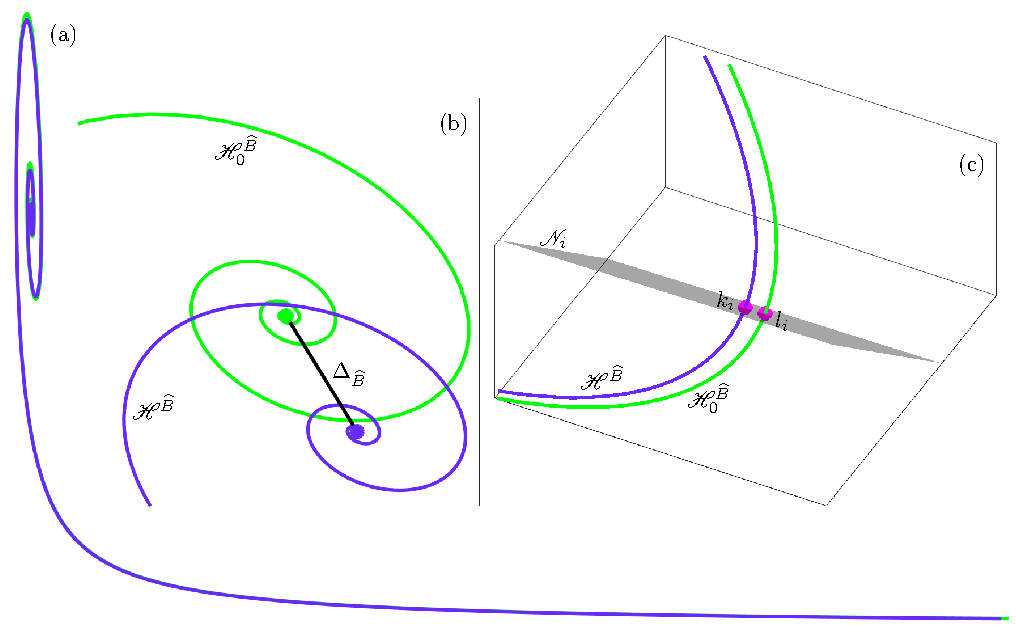
\includegraphics[]{./figures/MKMO_21.pdf}
\caption{Intersection curves $\mathscr{H}^{\widehat{B}}$ (royal purple) and $\mathscr{H}_0^{\widehat{B}}$ (green) for $\widehat{B}=0.75$ projected onto the ($A$, $X$)-plane (a).  An enlargement of the spiralling region near the end points of the curves is shown in panel (b) with the line of length $\Delta_{\widehat{B}}$ connecting them.  Panel (c) shows a further enlargement of the spiralling region inside the section $\Lambda$, represented by  ($A$, $X$, $Y$)-space, with the plane $\mathscr{N}_i$ (charcoal surface) that is normal to $\mathscr{H}_0^{\widehat{B}}$ at the point $l_i$ (magenta dot).  The corresponding point $k_i$ on $\mathscr{H}^{\widehat{B}}$ is also shown in magenta.}
\label{figure_21}
\end{figure}

Figure \ref{figure_21}(a) shows $\mathscr{H}_0^{\widehat{B}}$ (green curve) with $\mathscr{H}^{\widehat{B}}$ (purple curve) plotted after for $\widehat{B}=0.75$  projected onto the ($A$, $X$)-plane.  Note that before truncation, the right-hand end point of $\mathscr{H}_0^{\widehat{B}}$ extends past $\mathscr{H}^{\widehat{B}}$ in the ($A$, $X$)-projection.  In panel (b), the distance $\Delta_{\widehat{B}} \approx 0.009796$, between the boundary points on the spiralling end of $\mathscr{H}_0^{\widehat{B}}$ (green dot) and $\mathscr{H}^{\widehat{B}}$ (purple dot) is represented by a connecting black line.  We truncate the curve $\mathscr{H}_0^{\widehat{B}}$ as above.  With the built in \textsc{Matlab} function \textsc{spline}, we fit splines $Spl_0$ and $Spl$ to the truncated curves $\mathscr{H}_0^{\widehat{B}}$ and $\mathscr{H}^{\widehat{B}}$, respectively.  We choose the set of $N=751$ computed data points obtained from the $\textsc{Auto}$ continuation as the mesh on $\mathscr{H}_0^{\widehat{B}}$.  For each data point $l_i$, we compute $\mathscr{N}_i$ by applying the built-in \textsc{Matlab} function \textsc{fnder} to $Spl_0$ to obtain a unit tangent vector.  The tangent vector is then used to define two normal vectors that span $\mathscr{N}_i$.  Points $k_i$ are chosen to be the intersection of the function $Spl$ with $\mathscr{N}_i$. Figure \ref{figure_21}(c) shows a further enlargement of $\mathscr{H}_0^{\widehat{B}}$ and $\mathscr{H}^{\widehat{B}}$, where a representative ($l_i$, $k_i$)-pair (magenta dots) is shown with the corresponding $\mathscr{N}_i$ (charcoal plane).

Our approach works for almost all points.  The surface $\mathscr{N}_1$ has a unique intersection with $\mathscr{H}^{\widehat{B}}$, so our choice is well defined for $i=1$.  One challenge we encounter for larger $i$ is that some $\mathscr{N}_i$ have several intersections with $\mathscr{H}^{\widehat{B}}$.  For these values of $i$ we choose $k_i$ to be the intersection with the smallest arclength distance from $k_{i-1}$.  Another challenge is that some $\mathscr{N}_i$ do not intersect $\mathscr{H}^{\widehat{B}}$ at an appropriate location due to tangencies of the perpendicular planes with $\mathscr{H}^{\widehat{B}}$.  In these cases, $\mathscr{N}_i$ may intersect $\mathscr{H}^{\widehat{B}}$ several spirals ahead of $k_{i-1}$ or $\mathscr{N}_i$ may not intersect $\mathscr{H}^{\widehat{B}}$ at all.  For these $i$, we omit the point $l_i$ from our computation and lower the mesh size $N$ by one.    A final challenge is that some points $k_i$ are outside the convolute of $Spl_0$; however, we do include these points in our computation.

With this method, we find that the integral norm between $\mathscr{H}_0^{\widehat{B}}$ and $\mathscr{H}^{\widehat{B}}$ for $\widehat{B} = 0.75$ is approximately $7.64 \times 10^{-3}$.

The above computation is repeated for the remaining values of $\widehat{B}$, mentioned in Figure \ref{figure_20}, and the results are summarized in Table 2.
  
\begin{table}[h]
    \tbl{Integral norms between $\mathscr{H}_0^{\widehat{B}}$ and $\mathscr{H}^{\widehat{B}}$ for several values of $\widehat{B}$.}
        {\begin{tabular}{c  c  c  c  c  c  c  c  c} \\[-2pt]
            \toprule
            $\widehat{B}$ & $0.4$ & $0.62$ & $0.75$ & $0.8$  \\[6pt]
            \hline\\[-6pt]
            $\Delta_{\widehat{B}}$ & $1.02414 \times 10^{-3}$ & $10.90585 \times 10^{-3}$ & $9.79563 \times 10^{-3}$ & $6.97168 \times 10^{-3}$ \\[6pt]
            \hline\\[-6pt]
            $d\widehat{B}$ & $0.0460310 \times 10^{-2}$ & $1.47538 \times 10^{-2}$ & $0.763856 \times 10^{-2}$ & $1.109913 \times 10^{-2}$ \\[1pt]
            \botrule
        \end{tabular}}
\end{table}

Table 2 shows that the integral norms $d\widehat{B}$ between $\mathscr{H}_0^{\widehat{B}}$ and $\mathscr{H}^{\widehat{B}}$ are of same order as $\Delta_{\widehat{B}}$.  As $\widehat{B}$ increases, so does the difference between $\Delta_{\widehat{B}}$ and $d\widehat{B}$.  This is to be expected since $\mathscr{H}_0^{\widehat{B}}$ and $\mathscr{H}^{\widehat{B}}$ are spiralling around different points in these regions.  Having sampled the distances between $\mathscr{H}_0^{\widehat{B}}$ and $\mathscr{H}^{\widehat{B}}$ for four different $\Lambda$ $it appears that \Delta_{\widehat{B}}$ gives an upper limit of overall distance between the cures.




\newpage
\bibliography{elle}

\end{document}